\section{Evaluation}

	% -實驗方法,metric(PRR,throughput)
	% -device
	% -distance
	% -exposure duration
	% -background running

 In \autoref{sec:unsync}, we derive the probability of symbol loss and mixed frame. The value is affected by the transmitting frame rate ($T_{f,tx}$), receiving frame rate ($T_{f,rx}$), the read-out time of the camera ($T_r$) and the height of the LED in the received image ($H$). 
 Therefore, in this chapter we present the experimental results of our unsynchronized VLC system with respect to these factors. The performance metrics we use in the experiments are Packet Reception Rate (PRR) and throughput.

Each symbol represents 4-bit, and thus we have 16 symbols. The symbol-to-frequency mapping table is shown in \autoref{tab:symbol}.

\begin{table*}[!htb]
\centering
\caption{symbol-to-frequency mapping table}
  %\tabcolsep=0.03cm
  %\tabcolsep=0.1cm
  %\large
        \begin{tabular}{c|c|c|c}
        \hline symbol & seq\_num 0 & seq\_num 1 & seq\_num 2 \\ 
    ~     & frequency / pixel width  & frequency / pixel width & frequency / pixel width \\
  \hline \hline 
  preamble & 5657.3886 / 6& x & x \\ \hline
  symbol delimiter & 4849.1902 / 7 & x & x \\ \hline  
  EOF & 3771.5924 / 9& x & x \\ \hline 
  0000 & 3394.4331 / 10& 1305.5512 / 26& 808.1984 / 42\\ \hline 
  0001 & 3085.8483 / 11& 1257.1974 / 27& 789.4031 / 43\\ \hline 
  0010 & 2828.6943 / 12& 1212.2975 / 28& 771.4620 / 44\\ \hline 
  0011 & 2611.1024 / 13& 1170.4941 / 29& 754.3185 / 45\\ \hline 
  0100 & 2424.5951 / 14& 1131.4777 / 30& 737.9202 / 46\\ \hline 
  0101 & 2262.9554 / 15& 1094.9784 / 31& 722.2198 / 47\\ \hline 
  0110 & 2121.5207 / 16& 1060.7603 / 32& 707.1736 / 48\\ \hline 
  0111 & 1996.7254 / 17& 1028.6161 / 33& 692.7415 / 49\\ \hline 
  1000 & 1885.7962 / 18& 998.3627 / 34& 678.8867 / 50\\ \hline 
  1001 & 1786.5438 / 19& 969.8380 / 35& 665.5751 / 51\\ \hline 
  1010 & 1697.2165 / 20& 942.8981 / 36& 652.7756 / 52\\ \hline 
  1011 & 1616.3967 / 21& 917.4144 / 37& 640.4590 / 53\\ \hline 
  1100 & 1542.9241 / 22& 893.2719 / 38& 628.5987 / 54\\ \hline 
  1101 & 1475.8405 / 23& 870.3674 / 39& 617.1697 / 55\\ \hline 
  1110 & 1414.3471 / 24& 848.6082 / 40& 606.1487 / 56\\ \hline 
  1111 & 1357.7733 / 25& 827.9105 / 41& 595.5146 / 57\\ \hline
        \end{tabular}
        \label{tab:symbol}
\end{table*}

Here, we will revisit the derivation of $P_{miss}$ previously mentioned in \autoref{sec:unsync}. The previous equation only considered the case of a complete symbol loss. However, in reality, we should also consider if part of the symbol is outside the gray area in \autoref{fig:mix}. and if the outside part of the symbol is shorter than $H_{min} T_r$. In this case, the symbol cannot be demodulated and should be considered missing. That is, the outside part of the symbol is not sufficient large to be decoded. Here we assume $H_{min}$ be three times of the widest pixel width we use to transmit, which means we at least can see three black-white strips in the received image. We also deduct the time duration of the symbol delimiter transmission when that symbol is transmitted. Thus, the probability is given by
\begin{equation}
	%P_{\operatorname{miss}}^ \prime=\frac{T_{f,rx} - (H - FD\_width)T_r - T_{f,tx} + max\_pixel * T_r * 2}{T_{f,rx}} \qquad \textrm{.}
	P_{\operatorname{miss}}^ \prime=\frac{T_{f,rx} - (H - H_{SD}) T_r +  2H_{min} Tr- T_{f,tx} }{T_{f,rx}} \qquad \textrm{.}
\end{equation}

\subsection{Performance under Different Receiving Frame Rate}
First, we want to show the improvement of the decoding performance due to the design of the symbol delimiter, the sequence number, and the parity symbol. We use a Bridgelux LED Array as the transmitter and the PointGrey Flea3 camera configured with 30 fps, as the receiver. \autoref{fig:exp1_setup} shows a photo illustrating our setup. 

We alter the receiving frame rate to obtain different tx/rx frame rate ratios from 0.9 to 2 to force unsynchronized transmitter and receiver pairs. That is, we fix the transmitting frame rate at 30 fps, and alter the receiving frame rate from 15 fps to 33 fps. We randomly generate 20 string sequences for each of the three settings: (1) no additional schemes; (2) with only symbol delimiter; and (3) with symbol delimiter, sequence number,  and parity symbol. 
The length of the string sequence is 20 bytes. Note that we also record the videos at random starting time to introduce random phase difference between the transmitter and the receiver.

\begin{figure}[!htb]
  \centering
  %\hspace{-5em}
  \includegraphics[scale=0.0375]{fig/exp1_setup.JPG}
  \caption{Experimental setup photo.}
  \label{fig:exp1_setup}
\end{figure}

\autoref{fig:exp1_1} shows the result. When the receiving frame rate and the transmitting frame rate are very close to each other, the first setting has slightly lower PRR, as a number of received image frame will be mixed with two symbols and a portion of them will be demodulated correctly. The other two settings perform similarly. 
However, as the difference between the frame rates increase, the differences in PRRs become very obvious. 


\begin{figure}[!htb]
  %\centering
  \hspace{-2em}
  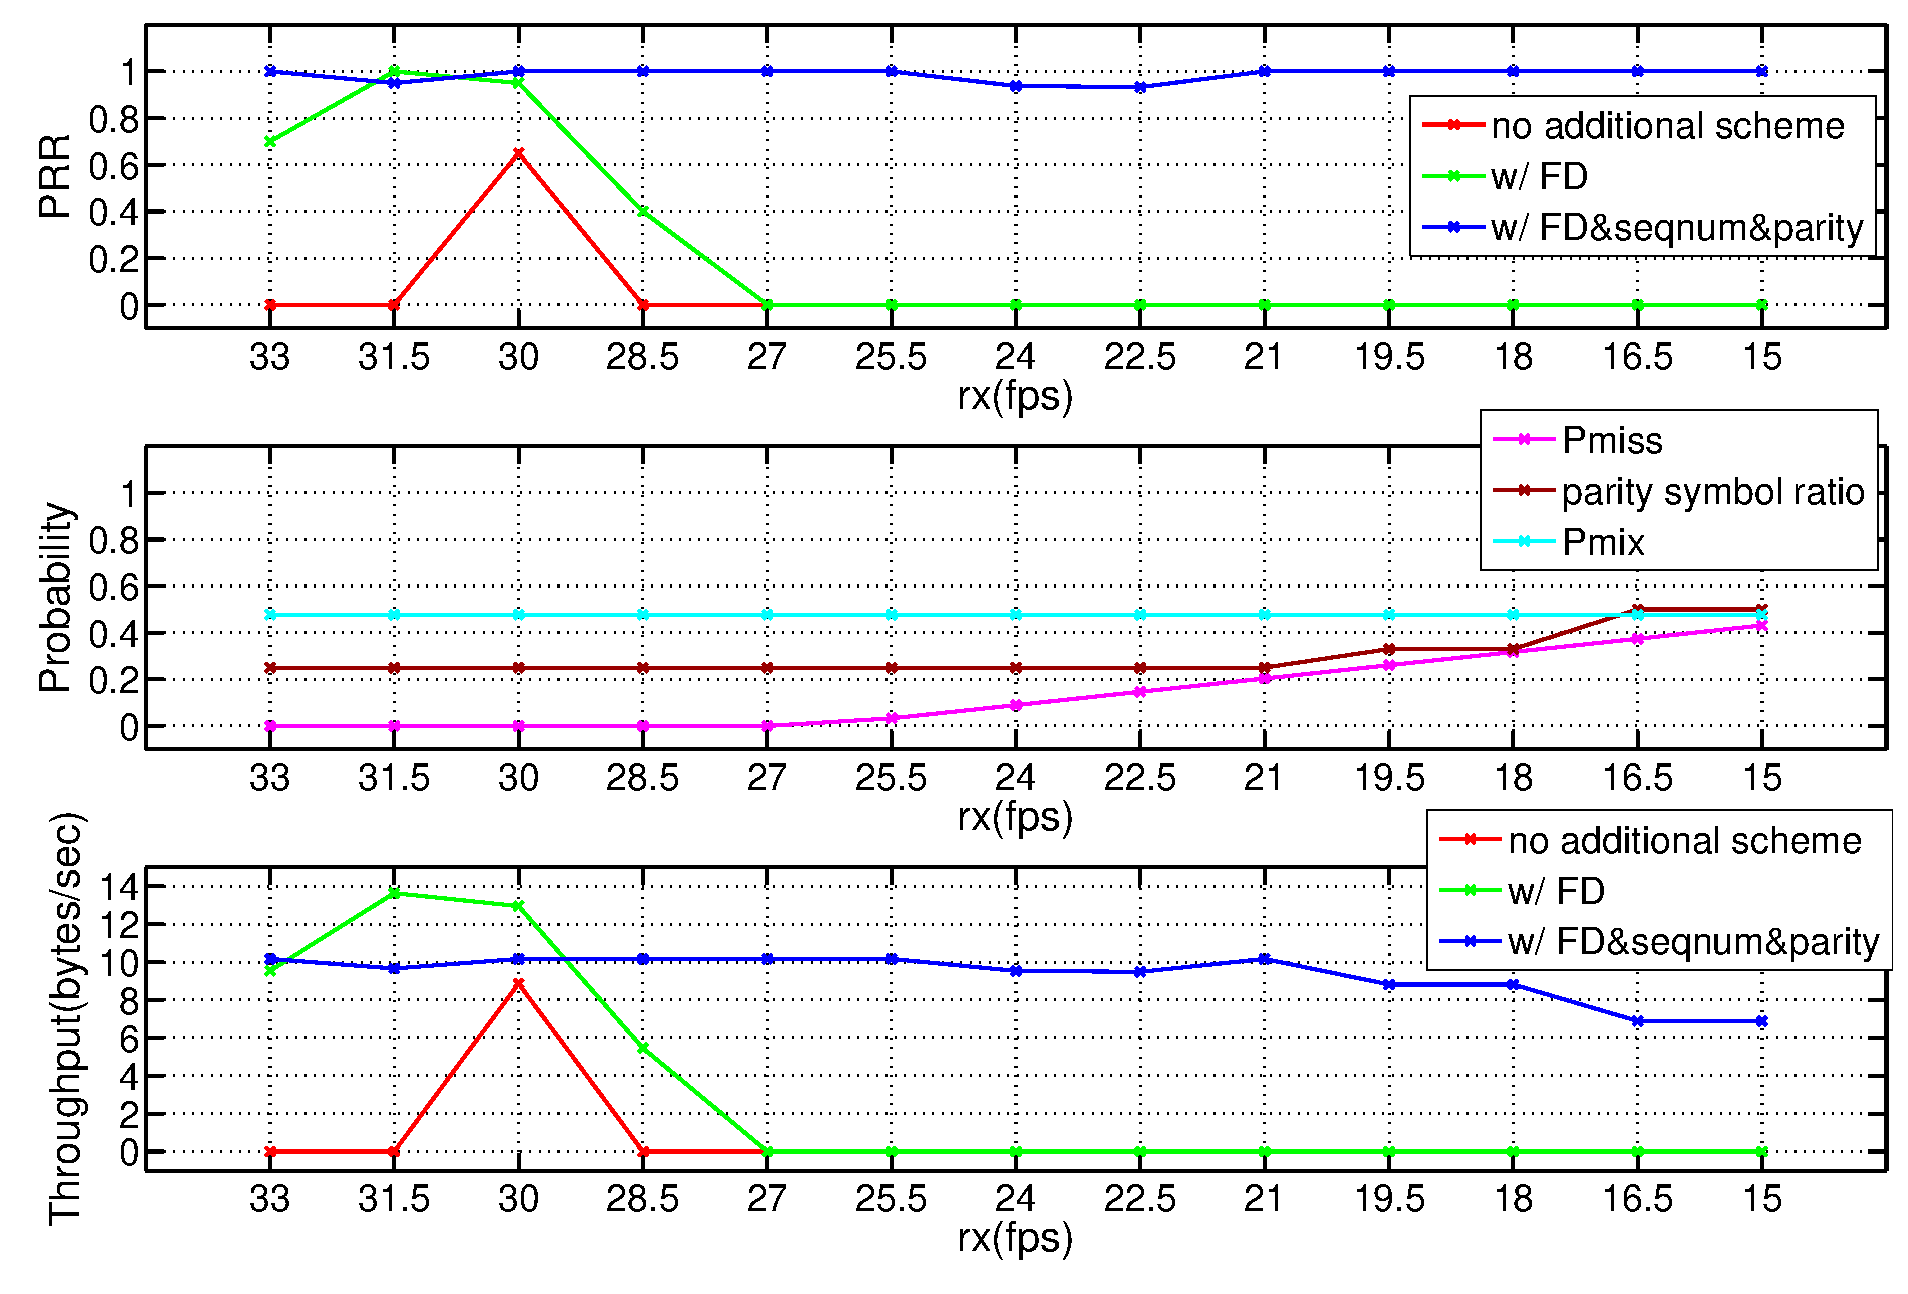
\includegraphics[scale=0.25]{fig/exp1_new.eps}
  \caption{Result under different rx fps.}
  \label{fig:exp1_1}
\end{figure}

The $P_{miss}^ \prime$ and parity symbol ratio are also shown in \autoref{fig:exp1_1}. 
For the third setting, we use $P_{miss}$ to determine the number of parity symbols required to be inserted into a packet. When the receiving frame rate is higher than 19.5 fps, the parity symbol ratio is configured to be 0.25, which means for every three symbols, we add a parity symbol. (It is possible to use a parity symbol rate less than 0.25, following the pink line in the figure. However, we do not discuss such a case here, and will discuss the maximum throughput in \autoref{sec:maxthroughput}.) When the receiving frame rate is between 19.5 and 18 fps, we use a parity symbol ratio of 0.33. When the receiving frame rate is lower than 18 fps, we use a parity symbol ratio of 0.5, which means for every symbol, we transmit twice.
With all 3 schemes, close to 100\% of the packets are received correctly, while the other two settings rapidly lose the ability to receive correct packets when the difference between frame rates increases. The results verify that our design can indeed address the issues caused by unsynchronized transmitter and receiver pair. 

We can see when the receiving frame rate and the transmission frame rate are close, the setting with the symbol delimiter has the highest throughput. As the difference between the frame rates increases, the throughput of the third setting decreases due to the large parity symbol ratio.

\subsection{Performance under Varying Inter-frame Interval}
According to~\cite{hu2013lightsync}, the receiving frame rate of smartphone cameras exhibit more variability for several reasons. Even when the average frame rate appears steady, the inter-frame interval still varies. 
In order to show the improvement with our new design scheme, we emulate this phenomena with a system with time varying inter-frame interval. 
However, it is hard to alter the receiving frame rate while receiving frames. We therefore use the Flea3 camera with fixed receiving frame rate and alter the transmitting frame rate before transmitting every symbol. 
To simulate the various of transmitting frame rate, we use a truncated normal distribution with the mean value of 36.9458 fps, the standard deviation of 3.94, the min value 31.03 fps and the max value 42.86 fps. 
The normal distribution of various transmitting frame rate is shown in \autoref{fig:norm}. 
The values are based on observations presented in~\cite{hu2013lightsync}, which states that the receiving frame rate fluctuates significantly between 21 to 29 fps for an entirely white foreground, with an average of around 25 fps. \autoref{fig:norm_vary} shows the generated random numbers for each transmitting frame.

\begin{figure}[!htb]
  \centering
  %\hspace{-5em}
  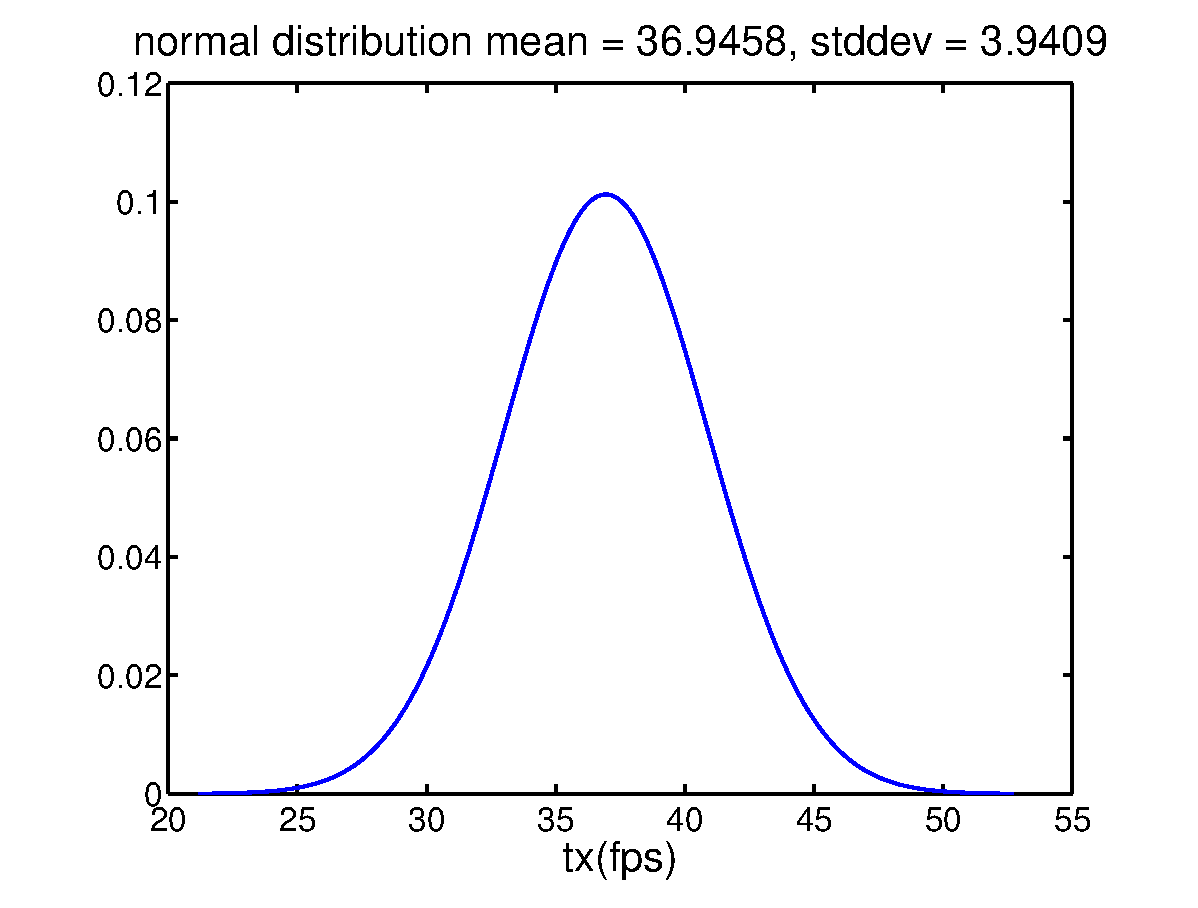
\includegraphics[scale=0.3]{fig/norm.eps}
  \caption{Normal distribution of various transmitting frame rate.}
  \label{fig:norm}
\end{figure}

\begin{figure}[!htb]
  \centering
  %\hspace{-5em}
  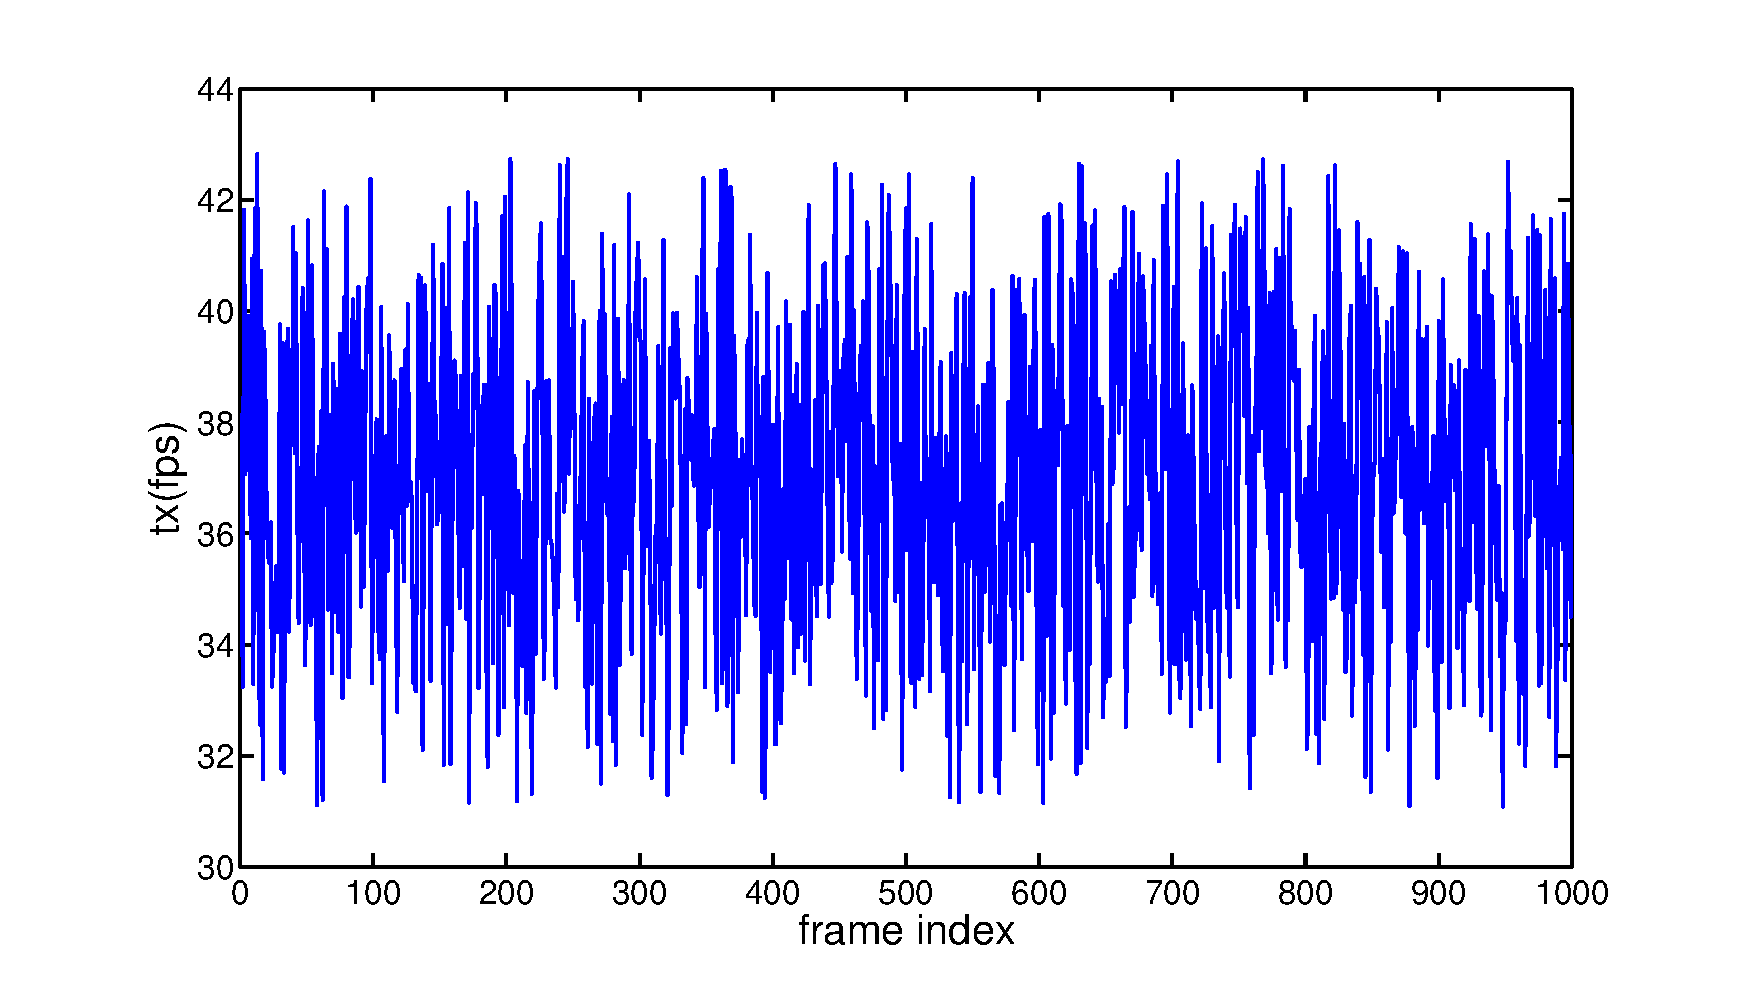
\includegraphics[scale=0.25]{fig/norm_vary.eps}
  \caption{Generated random numbers from the normal distribution in \autoref{fig:norm}.}
  \label{fig:norm_vary}
\end{figure}

We again generate 20 random string sequences. The length of each string sequence is 20 bytes. For each transmitting symbol, we randomly pick a number from the truncated normal distribution and transmit the symbol with the generated frame rate.
We use the PointGrey Flea3 camera to record the video at fixed 30 fps. 

\autoref{tab:norm_result} shows the result of PRR and throughput.
First, we want to know how frequently mixed frame or lost symbol occur. Thus, we use the average transmitting frame rate 36.9458 fps to calculate the probability. We get $P_{miss}$ = 0.0501 and $P_{mix}$ = 0.5877.
We can see that with no additional schemes, the PRR is 0 since there are a large number of mixed frames. With only the symbol delimiter setting, the PRR is still 0 because there is a non-zero probability to have missed symbol. With all three schemes, the PRR is 1. It is worth mentioning that we use a lower parity symbol ratio to increase the throughput in this experiment.

\begin{table}[!htb]
\centering
\caption{PRR and Throughput under various inter-frame interval.}
        %\tabcolsep=1cm
        %\tabcolsep=0.08cm
        \begin{tabular}{lcc}
        \hline Setting & PRR & Throughput\\ 
        \hline \hline
        No additional schemes & 0 & 0 bytes per second\\
        With only symbol delimiter   & 0 & 0 bytes per second \\
        With symbol delimiter, sequence number and parity symbol ratio 0.125 & 1 & 13.94 bytes per second\\
        With symbol delimiter, sequence number and parity symbol ratio 0.143 & 1 & 13.68 bytes per second\\
        With symbol delimiter, sequence number and parity symbol ratio 0.167 & 0.95 & 11.89 bytes per second\\
        With symbol delimiter, sequence number and parity symbol ratio 0.2 & 1 & 12.31 bytes per second\\
        %With frame delimiter, sequence number and parity symbol ratio 0.25 & 1 & 12.1134\\
        %With frame delimiter, sequence number and parity symbol ratio 0.33 & 1 & 10.8664 \\
        %With frame delimiter, sequence number and parity symbol ratio 0.5 & 1 & 8.4933 \\
        \hline
        \end{tabular}
        \label{tab:norm_result}
\end{table}

\subsection{Performance under Different Smartphone Cameras}
Third, we use several smartphones to compare the decoding performance under the three previous mentioned settings. \autoref{tab:smartphone_spec} lists the phones and their specifications. 

\begin{table}[!htb]
\centering
\caption{Summary of camera parameters of different smartphone devices.}
   \tabcolsep=0.08cm
    \begin{tabular}{c|c|c|c|c}
    \hline
        Device and Camera & Image Resolution & Frame Rate & Measured Read-out & Time Gap (ms)    \\
                    &   ($X_{\max}$ x $Y_{\max}$)                &  (fps)          &  Time ($\mu$s) &  (Percentage of       \\ 
                    &  &  &  &  Frame Duration)   \\ \hline \hline
    Point Grey Flea3 & 2048x1080          & 30         & 14.73                   & 17.42 (52.26\%) \\ \hline
    Apple iPhone 5s Back  & 1920x1080          & 29.98      & 19.64                   & 12.15 (36.42\%) \\ \hline
    Apple iPhone 5s Front & 1280x720          & 29.98      & 35.03                   & 8.13 (24.38\%) \\ \hline
   HTC New One Back     & 1920x1080          & 29.94        & 19.08                   & 12.8 (38.31\%) \\ \hline
    HTC New One Front  & 1920x1080            & 29.6      & 31.06                   & 0.24 (0.72\%)  \\ \hline
    Samsung Galaxy S4 Back    & 1920x1080             & 29.93      & 25.53                   & 5.84 (17.48\%) \\ \hline
    Samsung Galaxy S4 Front & 1920x1080             & 29.91      & 30.39                   & 0.61 (1.82\%) \\ \hline
    \end{tabular}
    \label{tab:smartphone_spec}
\end{table}

Note that the receiving frame rate of the smartphones are not fixed. Moreover, the read-out time and the resolution of the camera of smartphones are also different. These will affect the probabilities of symbol loss and mixed frame. We again generate 20 random string sequences. The length of each string sequence is 20 bytes. \autoref{fig:exp2_setup} shows a photo illustrating the experimental setup. In this experiment, we place a lampshade on the top of the LED to diffuse the light.

\begin{figure}[!htb]
  \centering
  %\hspace{-5em}
  \includegraphics[scale=0.0375]{fig/exp2_setup.JPG}
  \caption{Experimental setup photo.}
  \label{fig:exp2_setup}
\end{figure}

According to \autoref{tab:smartphone_spec}, the read-out time of the smartphones are not the same. This means different smartphone cameras may observe the different pixel width (signal period) under the same transmitting frequency. Therefore we use the preamble symbol to calibrate the $T_r$ to minimize the error of the period estimates of all subsequent symbols in the packet. \autoref{fig:exp2_tr} shows the pixel width of different smartphone cameras. We use the pixel width of Flea3 as the base (the X-axis), and the Y-axis represents the observed pixel width. Generally, the pixel width grows linearly. What we need to do is to calibrate the lines to fit the top black line. 

\begin{figure}[!htb]
 % \centering
  \hspace{-5em}
  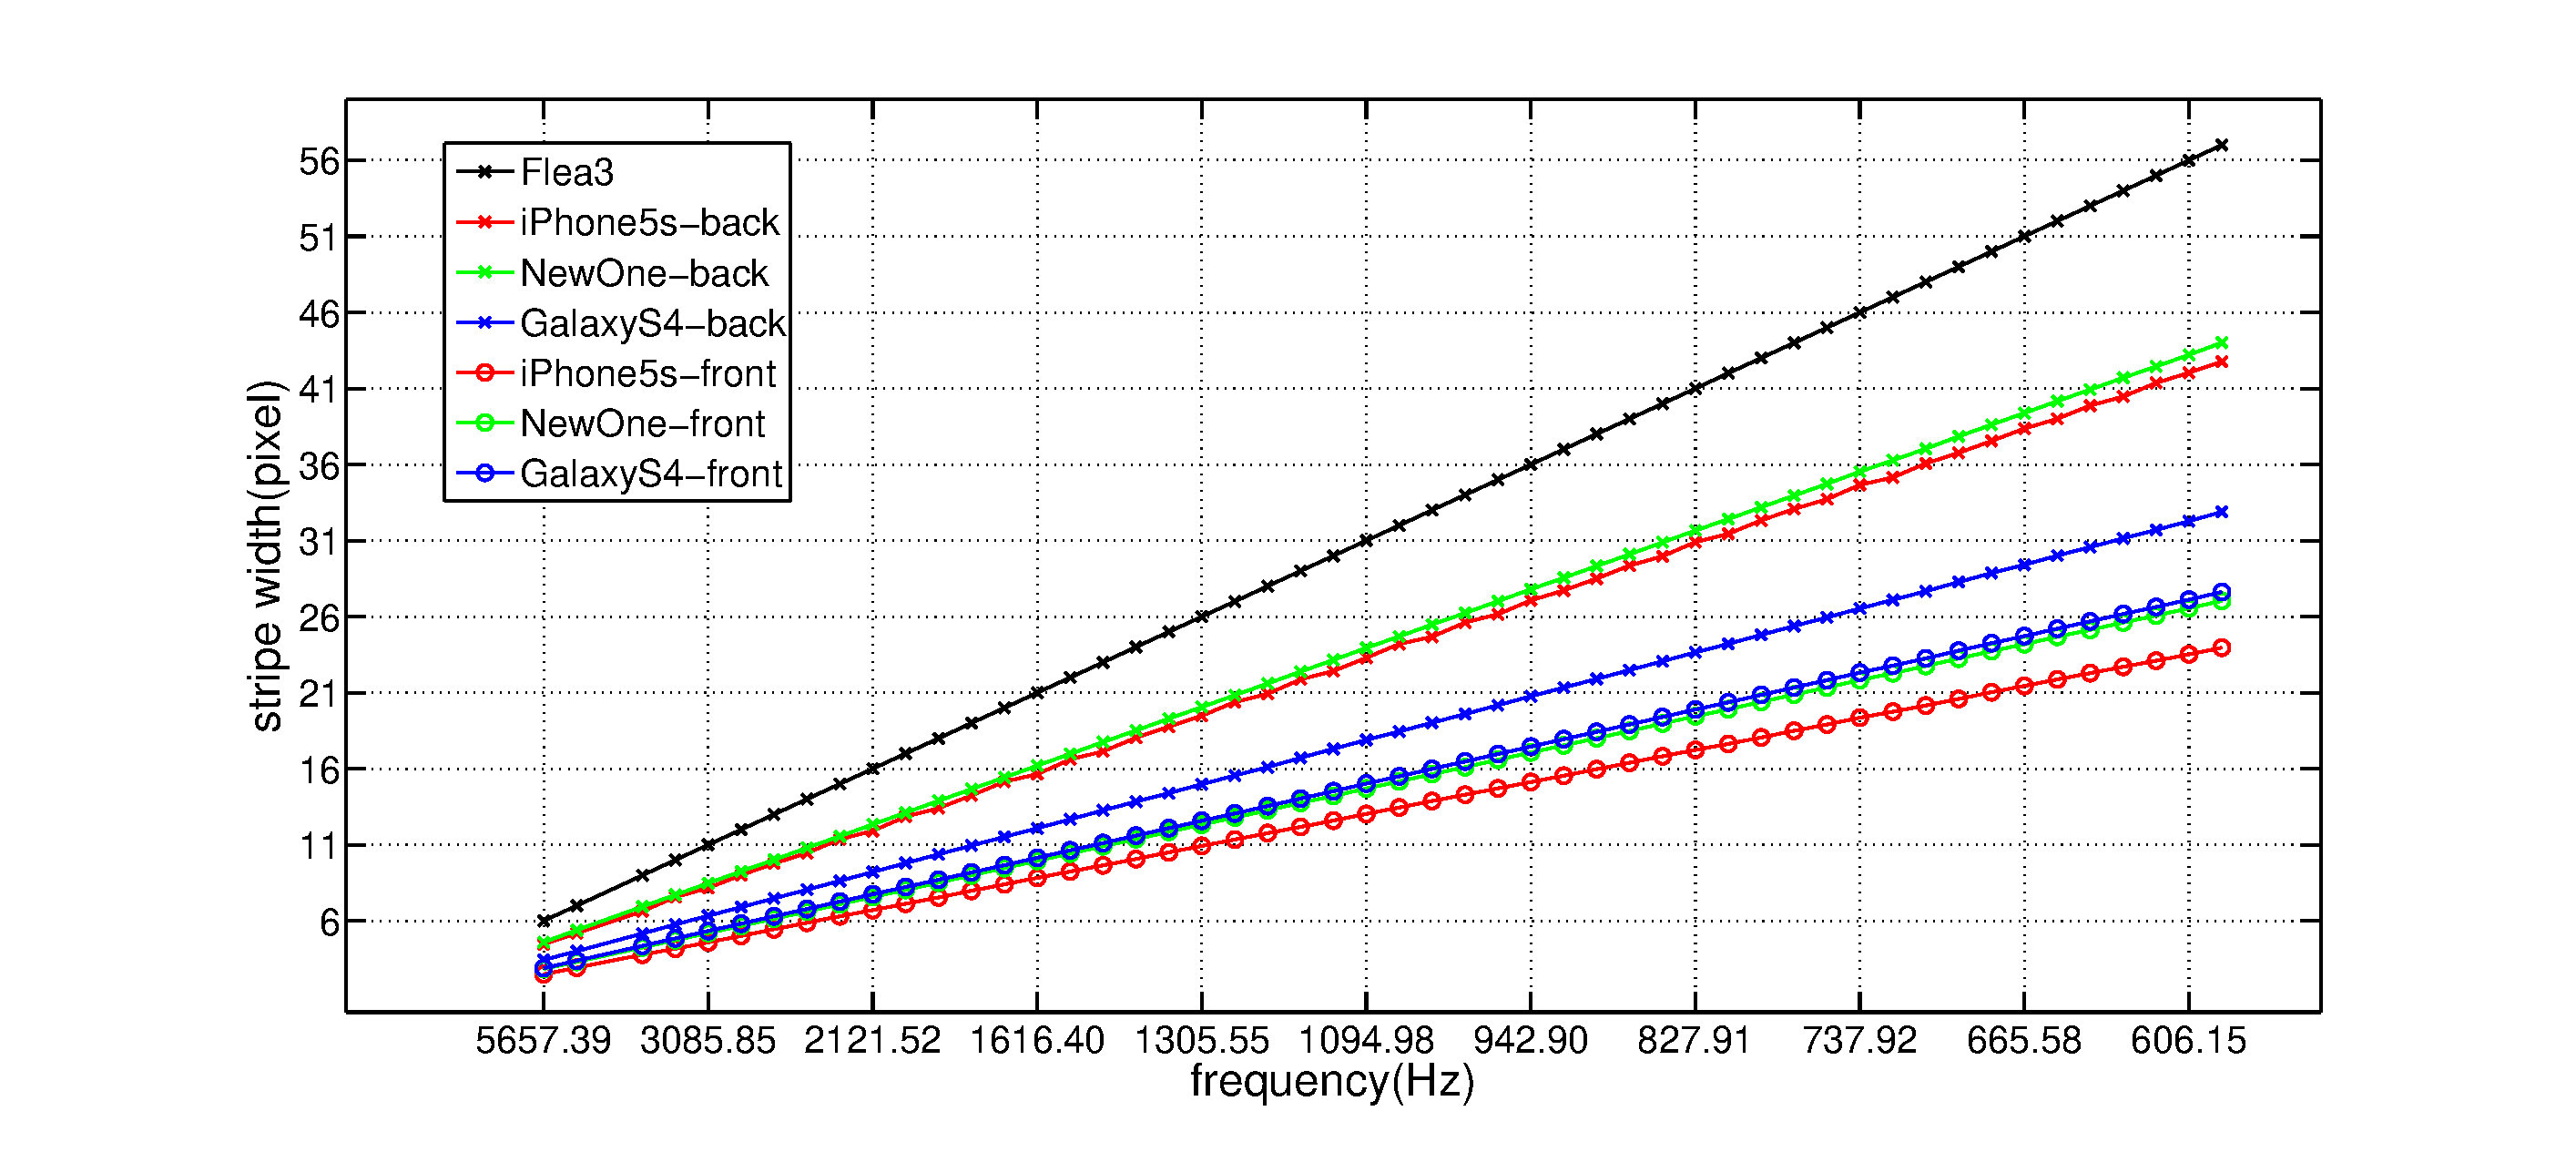
\includegraphics[scale=0.2]{fig/exp2_tr_new.eps}
  \caption{Pixel width under different smartphone devices.}
  \label{fig:exp2_tr}
\end{figure}

First, we use the preamble symbol for the calibration. After determining the pixel width of the preamble symbol, we calculate the ratio between the expected pixel width of our base - calculated with the images captured by Flea3 camera (which is around 6 pixel) and the pixel width calculated with the images captured by the smartphone camera. Then, for each received pixel width, we multiply the ratio and calculate the error. \autoref{fig:exp2_thin_diff} shows the absolute difference between the expected pixel width of Flea3 and the calibrated pixel width of smartphone devices. We can see as the pixel width grows, the error gets larger which can be as large as 1 pixel. If the error is larger than 0.5 pixel, it could be determined as a neighboring symbol and it would result in an erroneous symbol. The reason why the calibrated pixel width do not work well is that the camera sensor on the smartphones produce more noise in the image compared to the one of the Flea3. As a result, if the pixel width is too small (say, less than 15 pixel), it will have a higher error probability. The result implies that the pixel width of current preamble symbol is too small.

\begin{figure}[!htb]
 % \centering
  \hspace{-5em}
  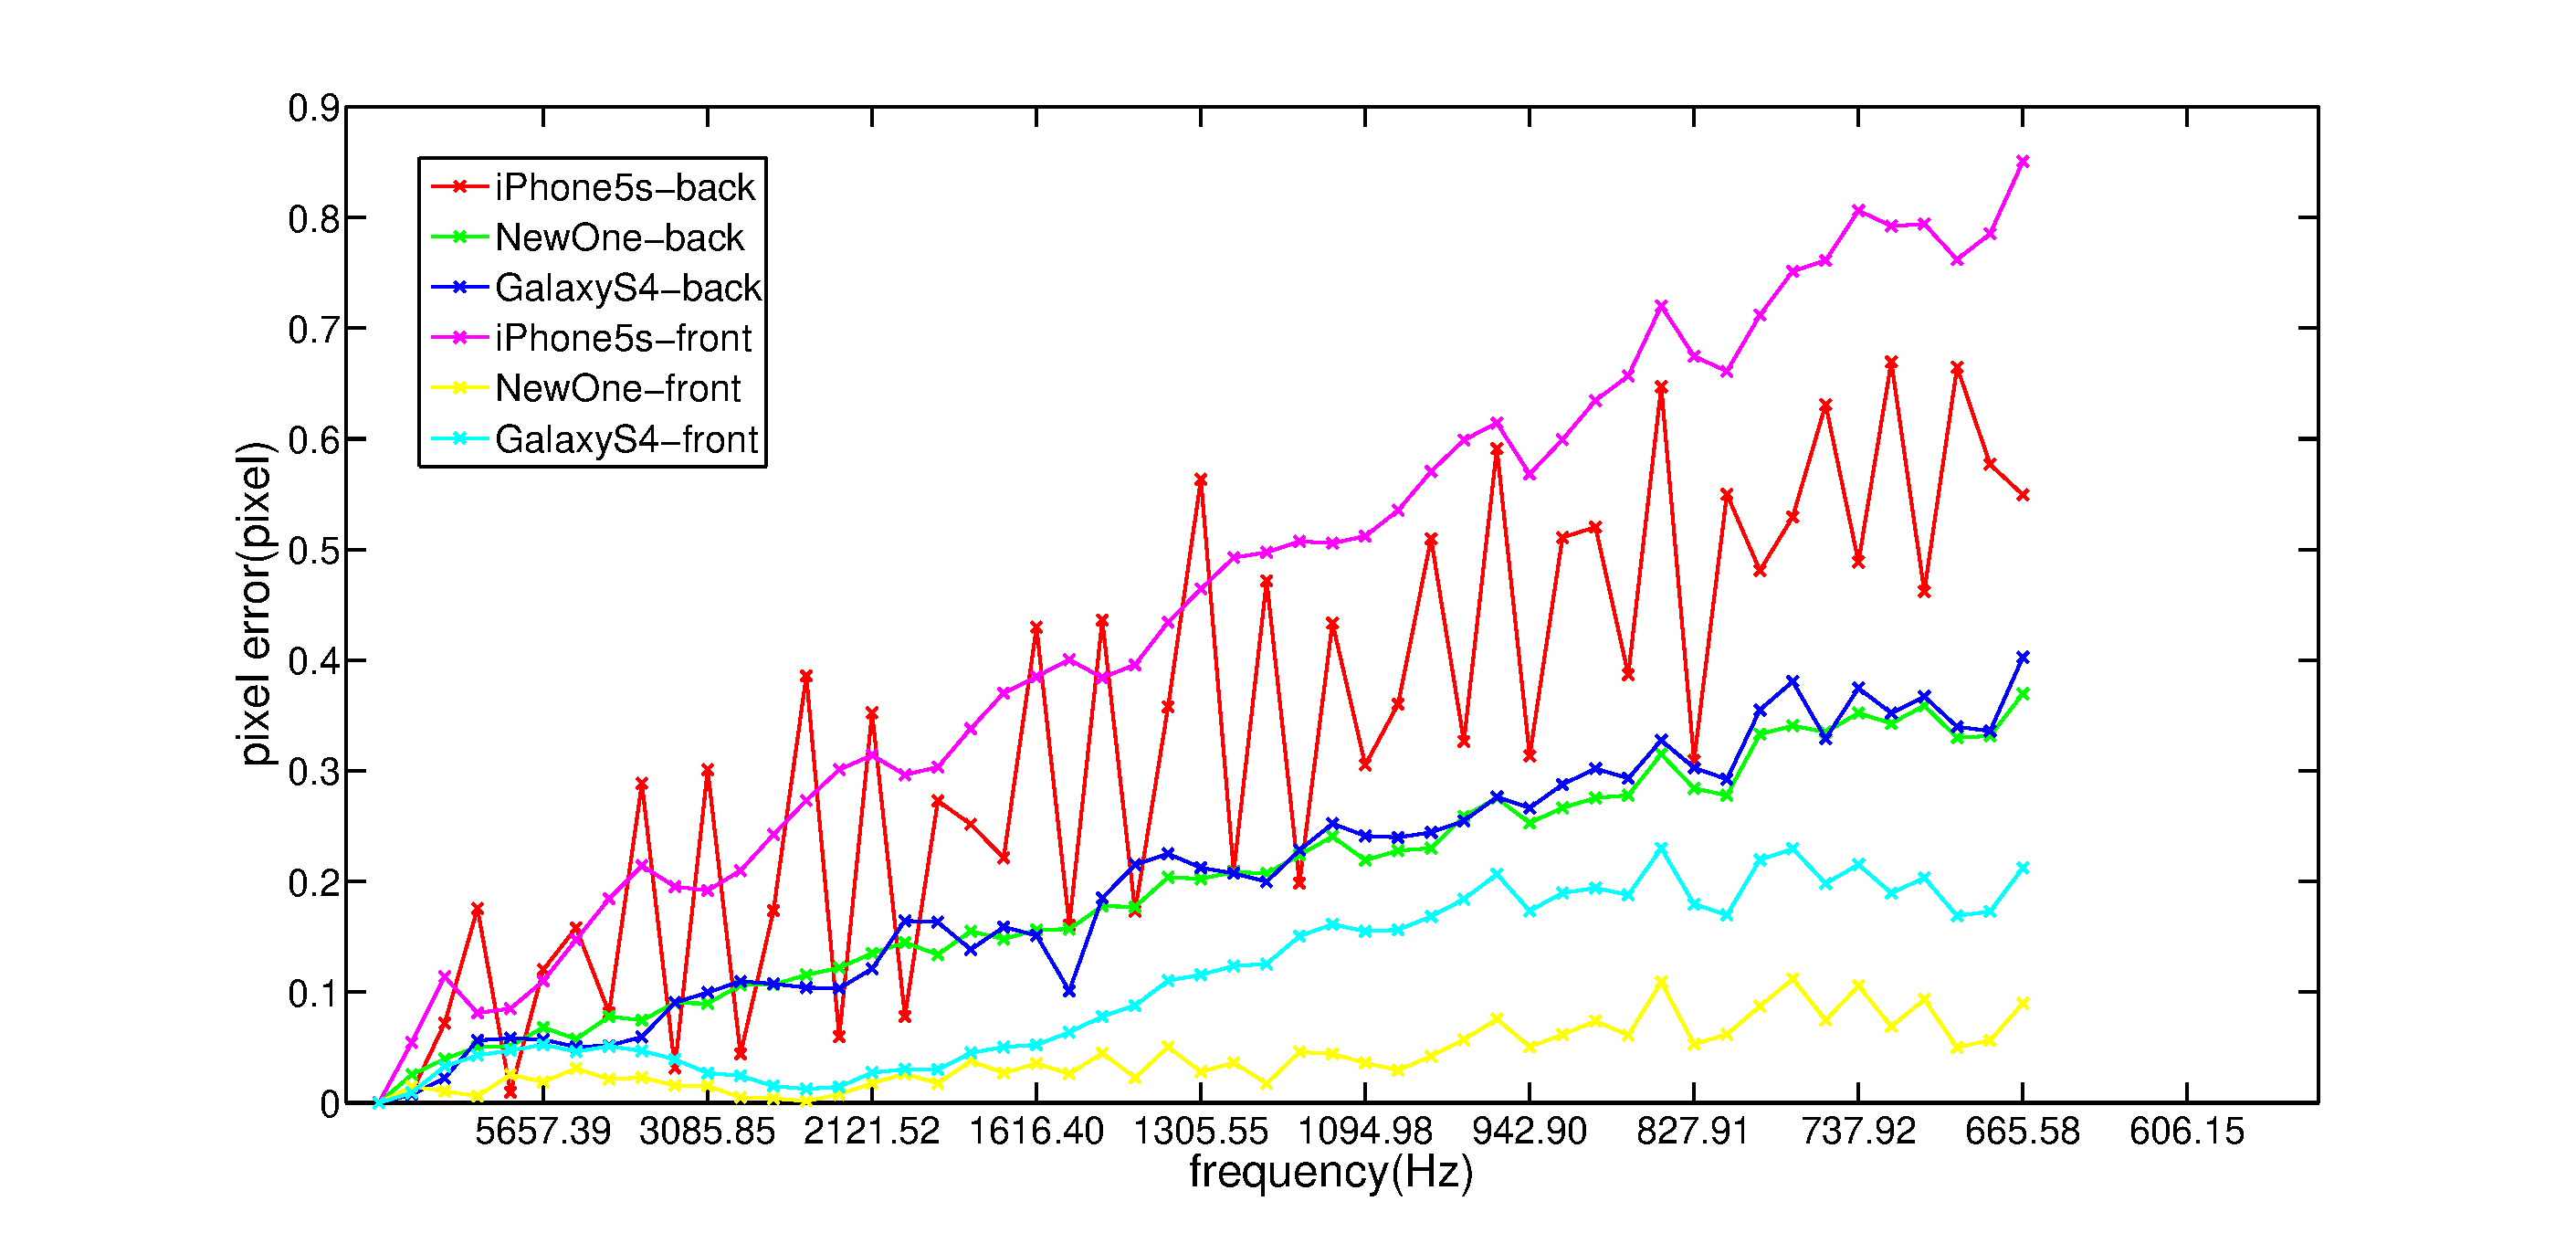
\includegraphics[scale=0.2]{fig/exp2_tr_error_thin.eps}
  \caption{Pixel error when using the symbol with the smallest signal period as the preamble.}
  \label{fig:exp2_thin_diff}
\end{figure}
\begin{figure}[!htb]
 % \centering
  \hspace{-5em}
  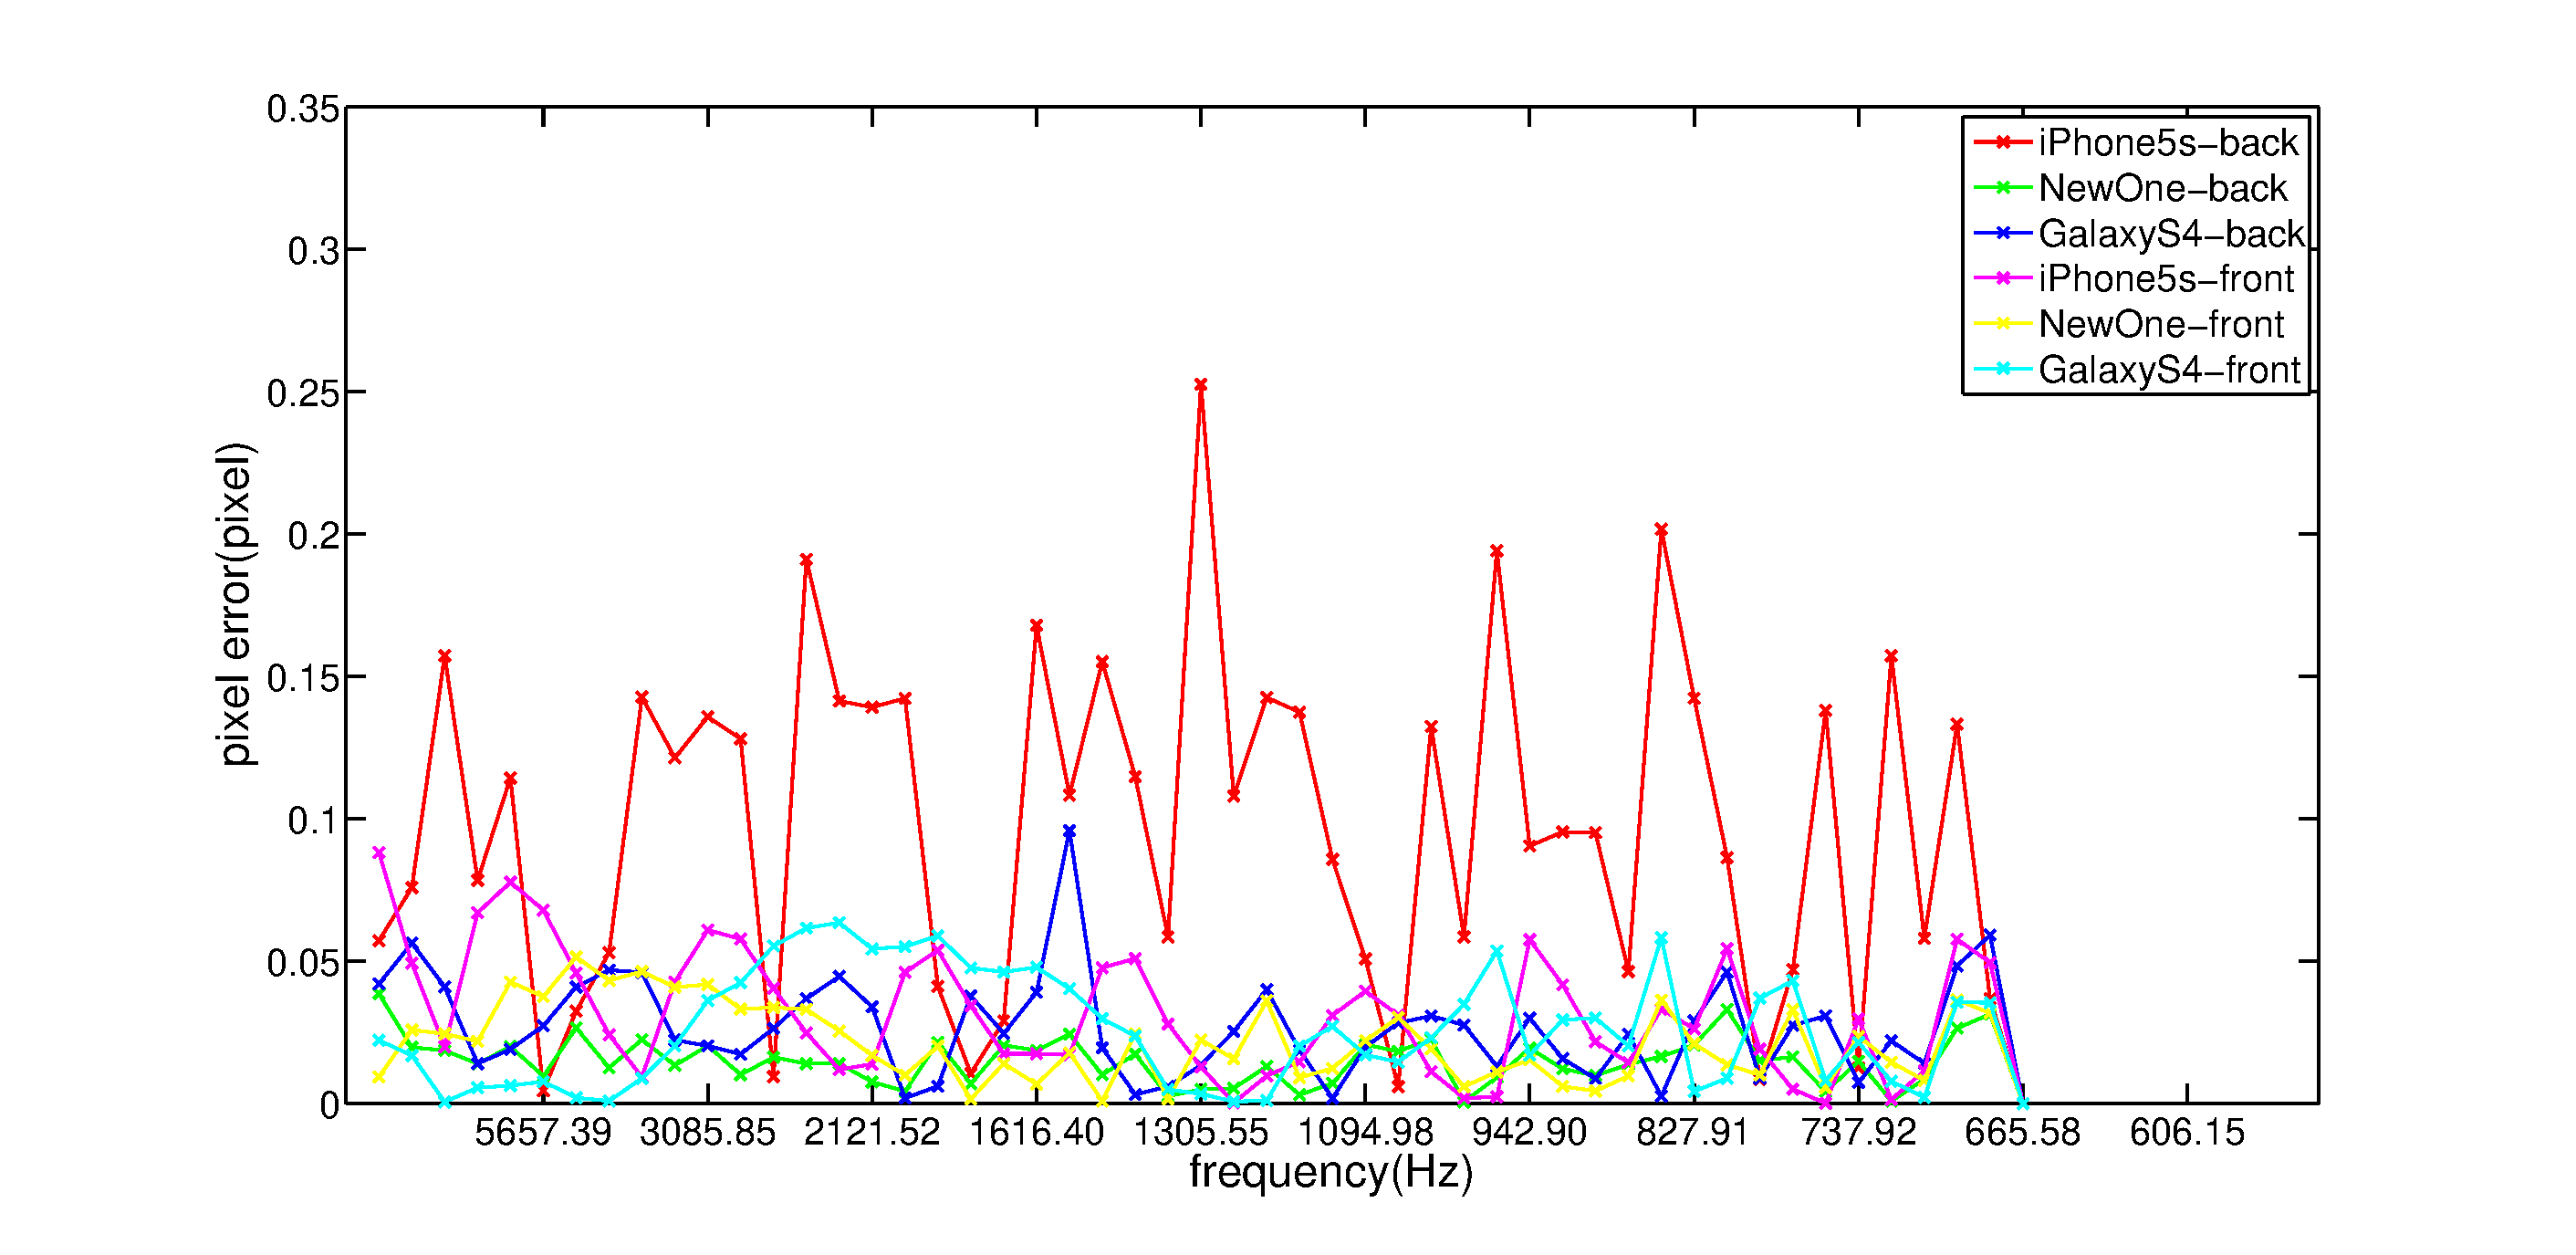
\includegraphics[scale=0.2]{fig/exp2_tr_error.eps}
  \caption{Pixel error when using the symbol with the largest signal period as the preamble.}
  \label{fig:exp2_fat_diff}
\end{figure}

To address this issue, we instead use the one with the largest pixel width as the preamble symbol. For the third setting, we use the frequency merely lower than the last transmitting symbol in \autoref{tab:symbol}, which is 585.24 Hz. With this symbol, the expected pixel width of Flea3 is around 58 pixel. We again calculate the ratio and the calibrated pixel width. \autoref{fig:exp2_fat_diff} shows the result of error. We can see that the pixel error of most devices is now smaller than 0.1 pixel. However, the back facing camera of the iPhone5s still has larger error, though also lower than 0.25 pixel, which is acceptable. For the first and second settings, we use the frequency lower than the last transmitting symbol, which is 1305.5512 Hz. With this symbol, the expected pixel width of Flea3 is around 26 pixel.


\autoref{fig:exp2_1} shows the result. The X-axis shows different smartphone cameras. We first calculate $P_{miss}$ by averaging the frame rate of each smartphone camera. The obtained values are all zeros since the average fps are close to 30. However, we can see that $P_{mix}$ is high. 

For the first setting, we can see the PRR is about 50\% to 60\%. The result also shows that when the $P_{mix}$ is higher, PRR of the first setting gets lower.
For the second and third settings, basically that PRRs are similar since no symbol miss take place. However, we can see that most of the devices show that the third setting gets lower PRR then the second setting. Some of the devices also show that the third setting gets lower PRR then the first setting. Furthermore, the overall PRR is on the low side. We think the problem is due to decoding error. Because of the instability of the smartphone cameras, if the received pixel width of the preamble has slightly error, it will affect the third setting very much because the pixel width range we use in the third setting is larger than the first two settings. The yellow and cyan bars in the figure represent the result ignoring the preamble error. We can see that PRRs of the second and third settings are very close to 1. (From this experiment, we can see that the second setting is good enough for the communications in spite of using different smartphones. However, the current setting uses regular video recording mode rather than preview mode, and the receiver is very close to the transmitter. That is, the are many factors not considered yet and these will be discussed in the following subsection.) Therefore, the error are mainly caused by the preamble calibration rather than the unsynchronized issues. To address the preamble calibration error, we can transmit more preamble symbols at the beginning of the packet and average them when receiving these symbols. This solution can minimize the error caused by calibration but will increase the packet overhead at the same time. 

\begin{figure}[!htb]
 % \centering
  \hspace{-3em}
  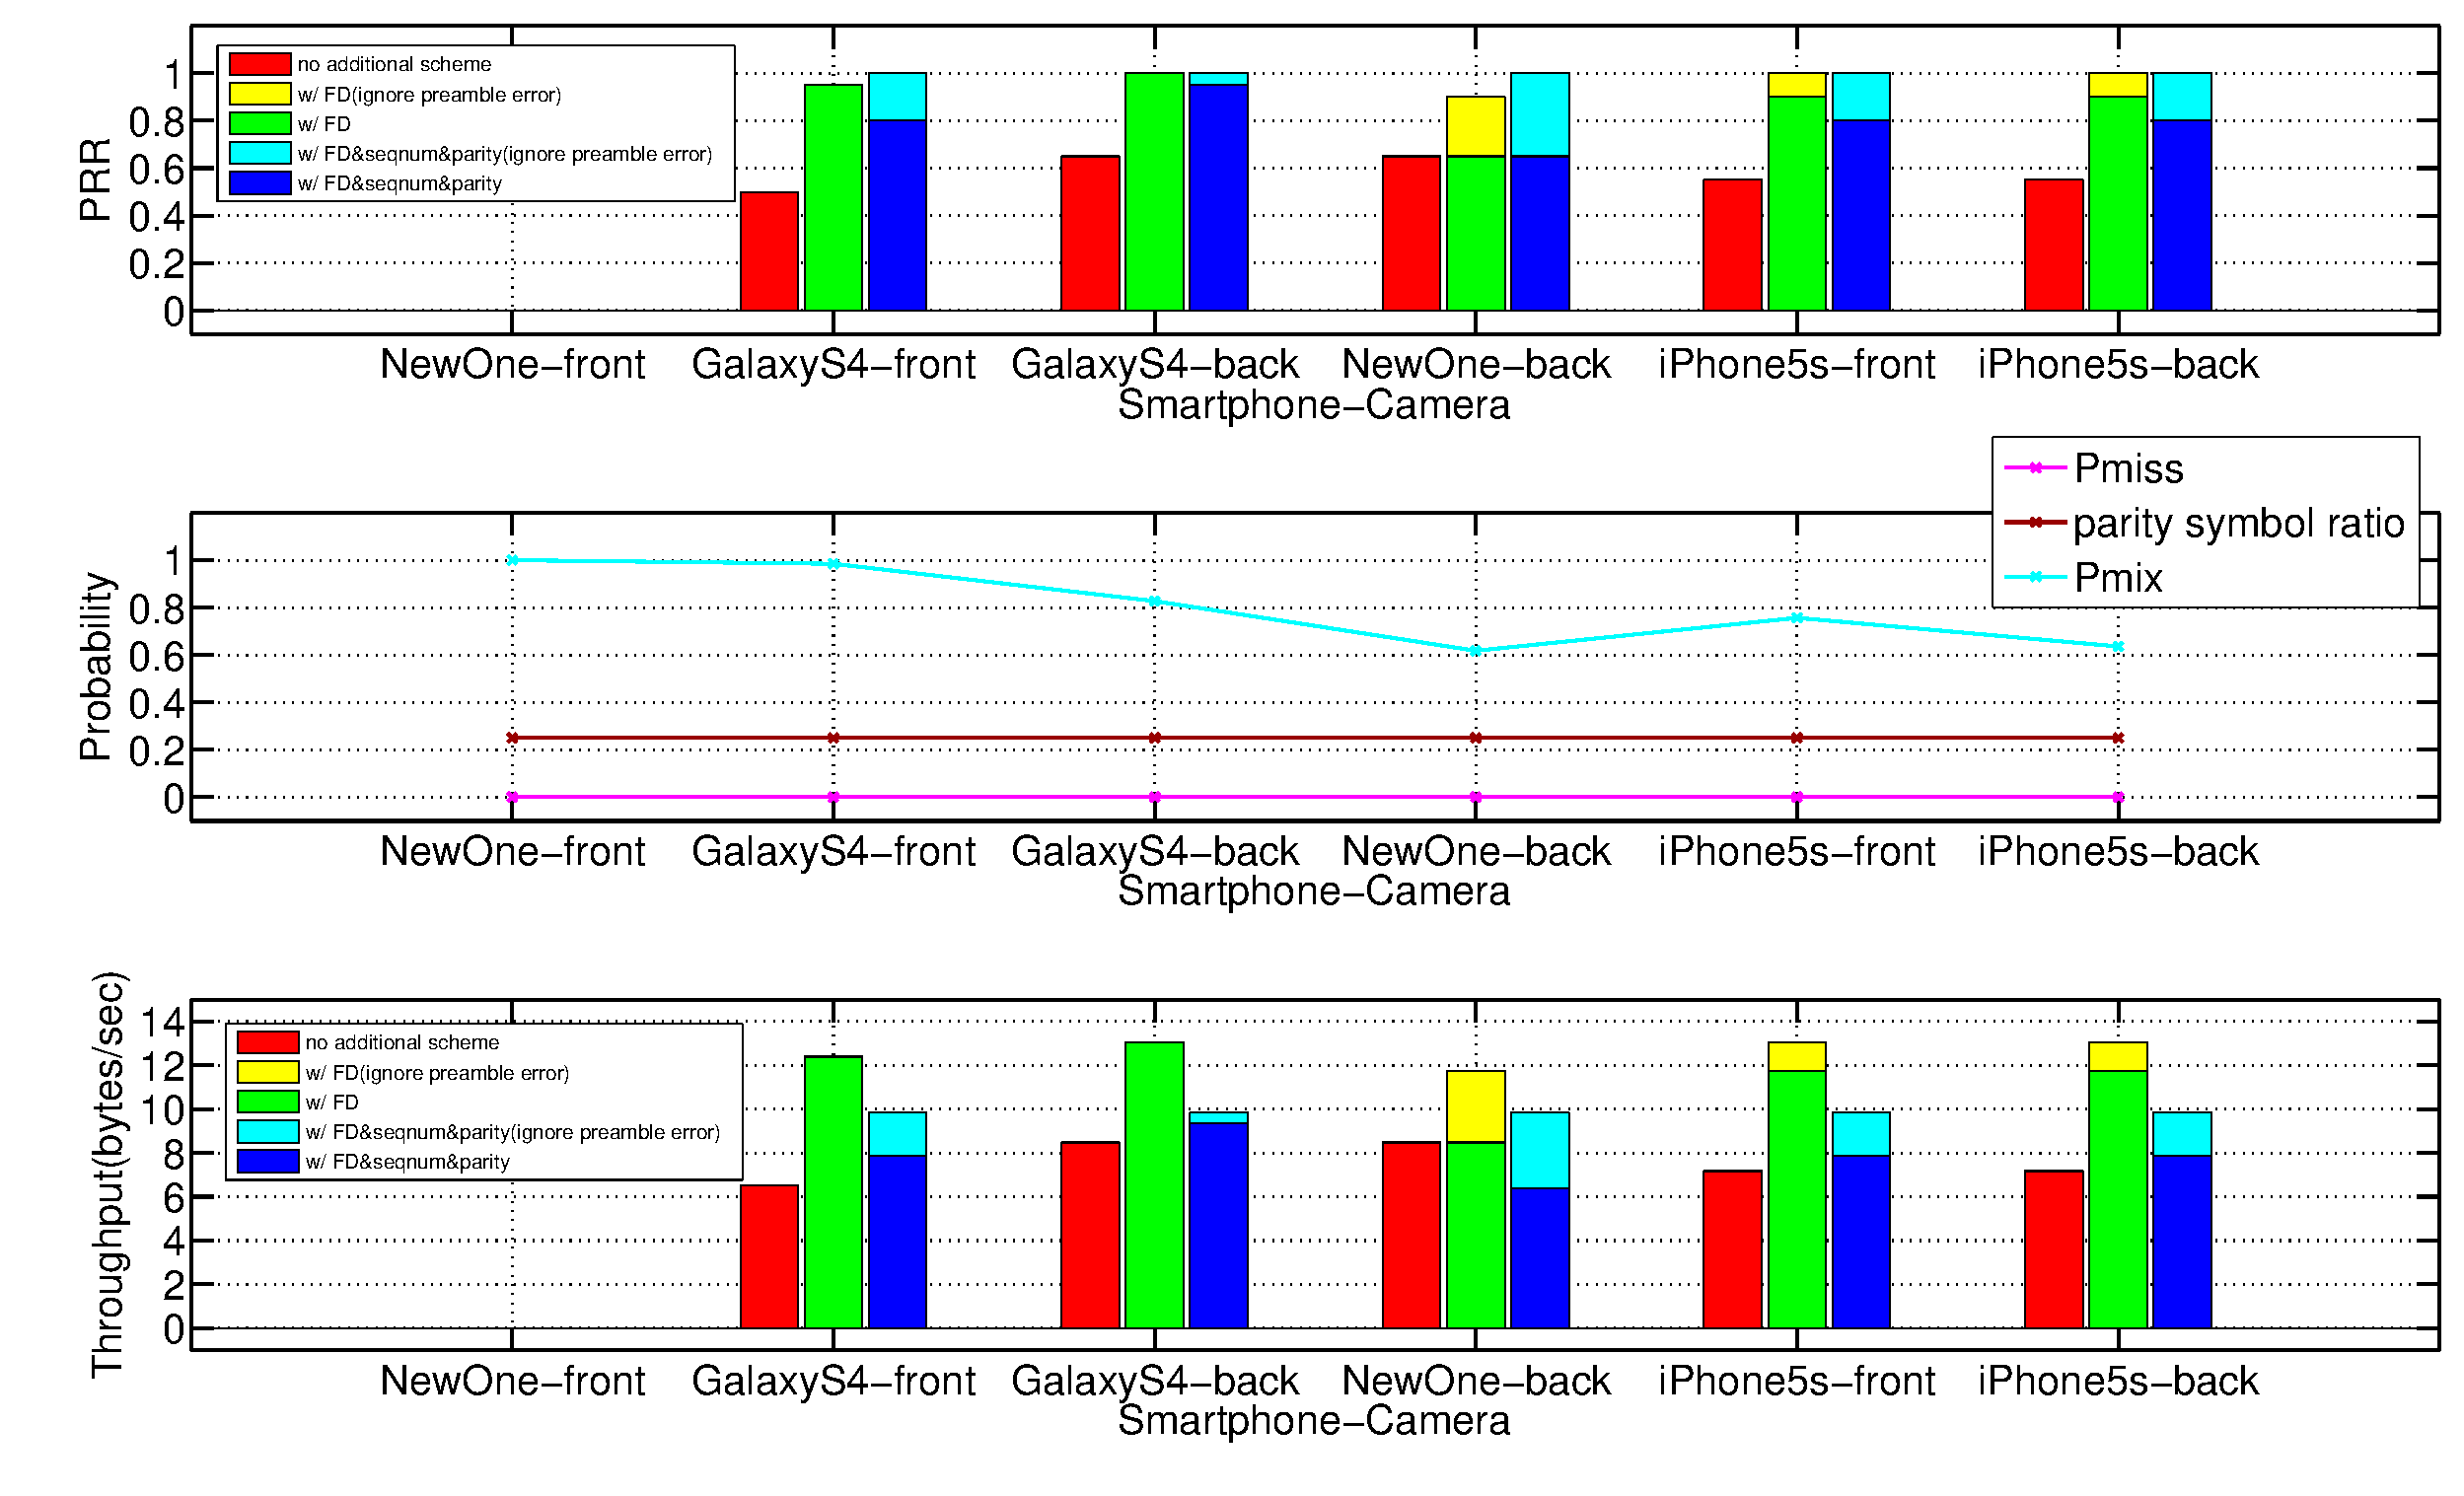
\includegraphics[scale=0.2]{fig/exp2_refine.eps}
  \caption{Result under different smartphone devices.}
  \label{fig:exp2_1}
\end{figure}

We also found that the front-facing camera of HTC NewOne cannot decode any packet in all three settings. We observed that the behavior of the camera records every frame twice. Even when we extract half of the frames in the video, it is still not able to decode.
Therefore, we think the problem is not related to our decoding method.
Our results indicate that, the second setting can obtain the maximum throughput in most settings.

\subsection{Max Throughput under Different Transmitting Frame Rate}
\label{sec:maxthroughput}
In this experiment, we fix the receiving frame rate and gradually increase the transmitting frame rate to determine the maximum achievable throughput, and when we can achieve it. As the transmitting frame rate gets higher, $P_{miss}$ increases, and thus we need to use a higher parity ratio to compensate. However, the transmitted data rate also increases. We would like to investigate at what transmitting frame rate the maximum throughput can be obtained.
In this experiment, we increase the transmitting frame rate from 33 fps to 90 fps. Two cameras are used in this experiment. The receiving frame rate of Flea3 is fixed at 30 fps. The iPhone5s is at 29.98 fps on average. We only use the third setting in this experiment.

\autoref{fig:exp3_1} shows the results of Flea3. We can see $P_{miss}$ grows from 0 to over 0.5, and the parity symbol ratio we select is just above the $P_{miss}$ line. Note that the parity symbol ratio we use is at most 0.5. Because we think the overhead costs too much if a symbol is transmitted over two times. We can see that PRR is more than 90\% until the transmitting frame rate reaches 81 fps. 
Theoretically, the upper limit of the transmitting frame rate is bounded by the case of having two symbols in a received frame, which is given by 
\begin{equation}
%Max\_tx\_fps = \frac{1}{(H - 2*FD\_width) T_r} \qquad \textrm{.}
FPS_{Max,tx}= \frac{1}{(H - 2H_{SD}) T_r} \qquad \textrm{.}
\end{equation}

The max transmitting frame rate for iPhone5s is about 53.39 fps, and 74.44 fps for the Flea3. However, two symbols in a received frame rarely happens. At that time the parity symbol can be used to recover data. Therefore, we can get even higher transmitting frame rate in practice.

\begin{figure}[!htb]
 %\centering
  \hspace{-2em}
  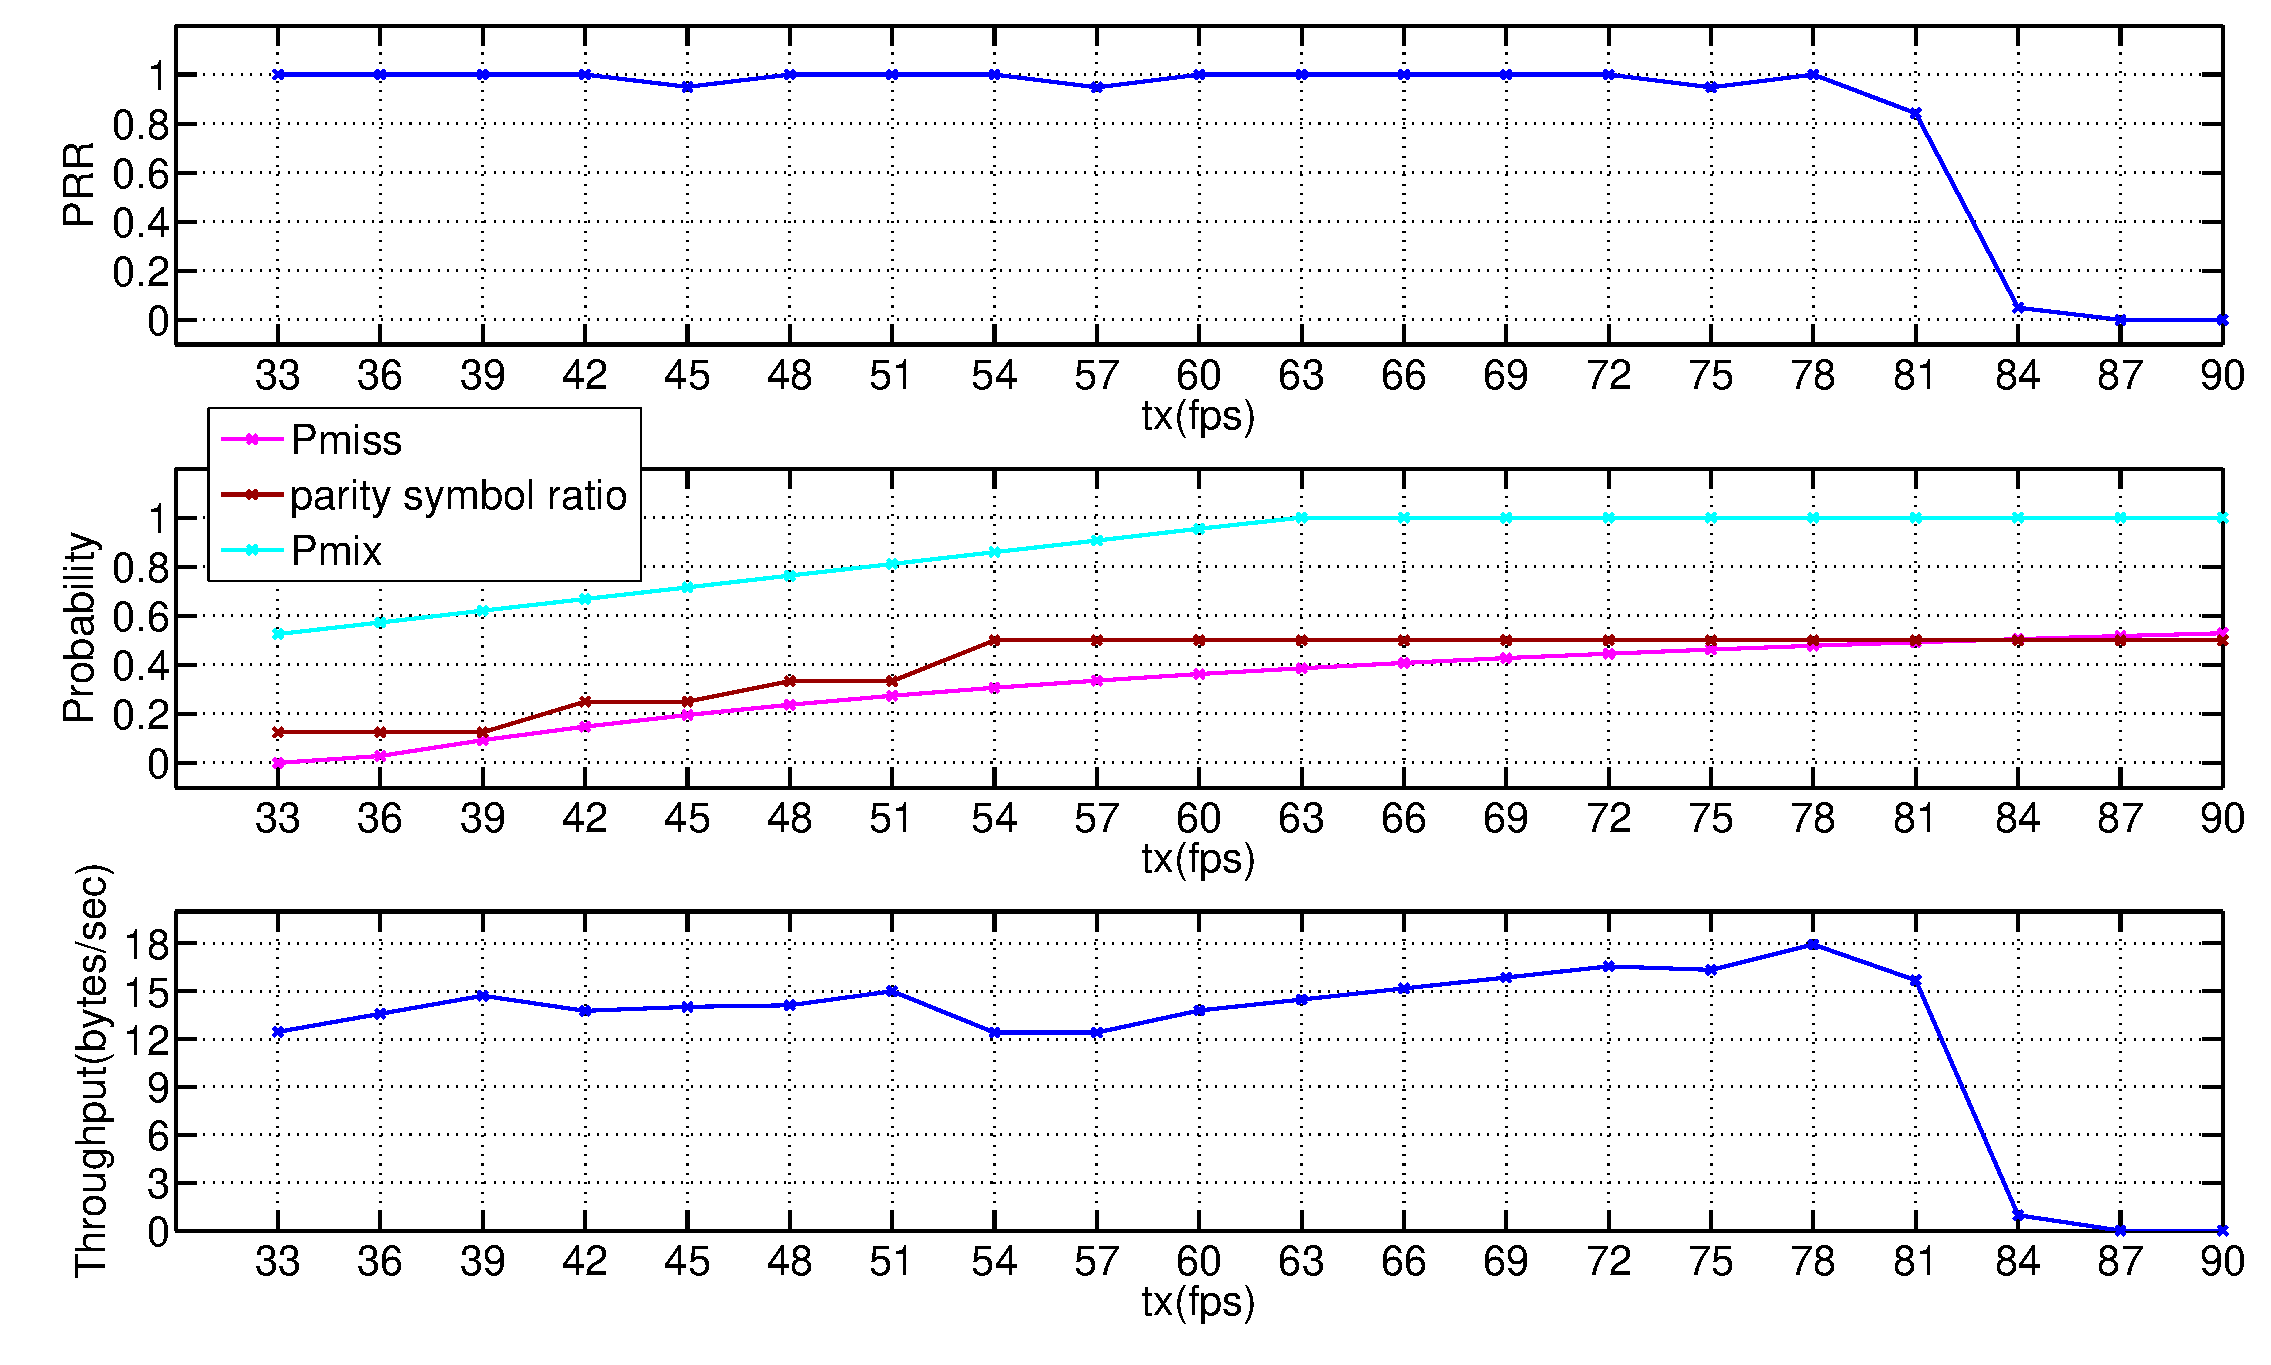
\includegraphics[scale=0.215]{fig/exp3_flea_new.eps}
  \caption{Result of Flea3 under different transmitting frame rate.}
  \label{fig:exp3_1}
\end{figure}

\begin{figure}[!htb]
 %\centering
  \hspace{-2em}
  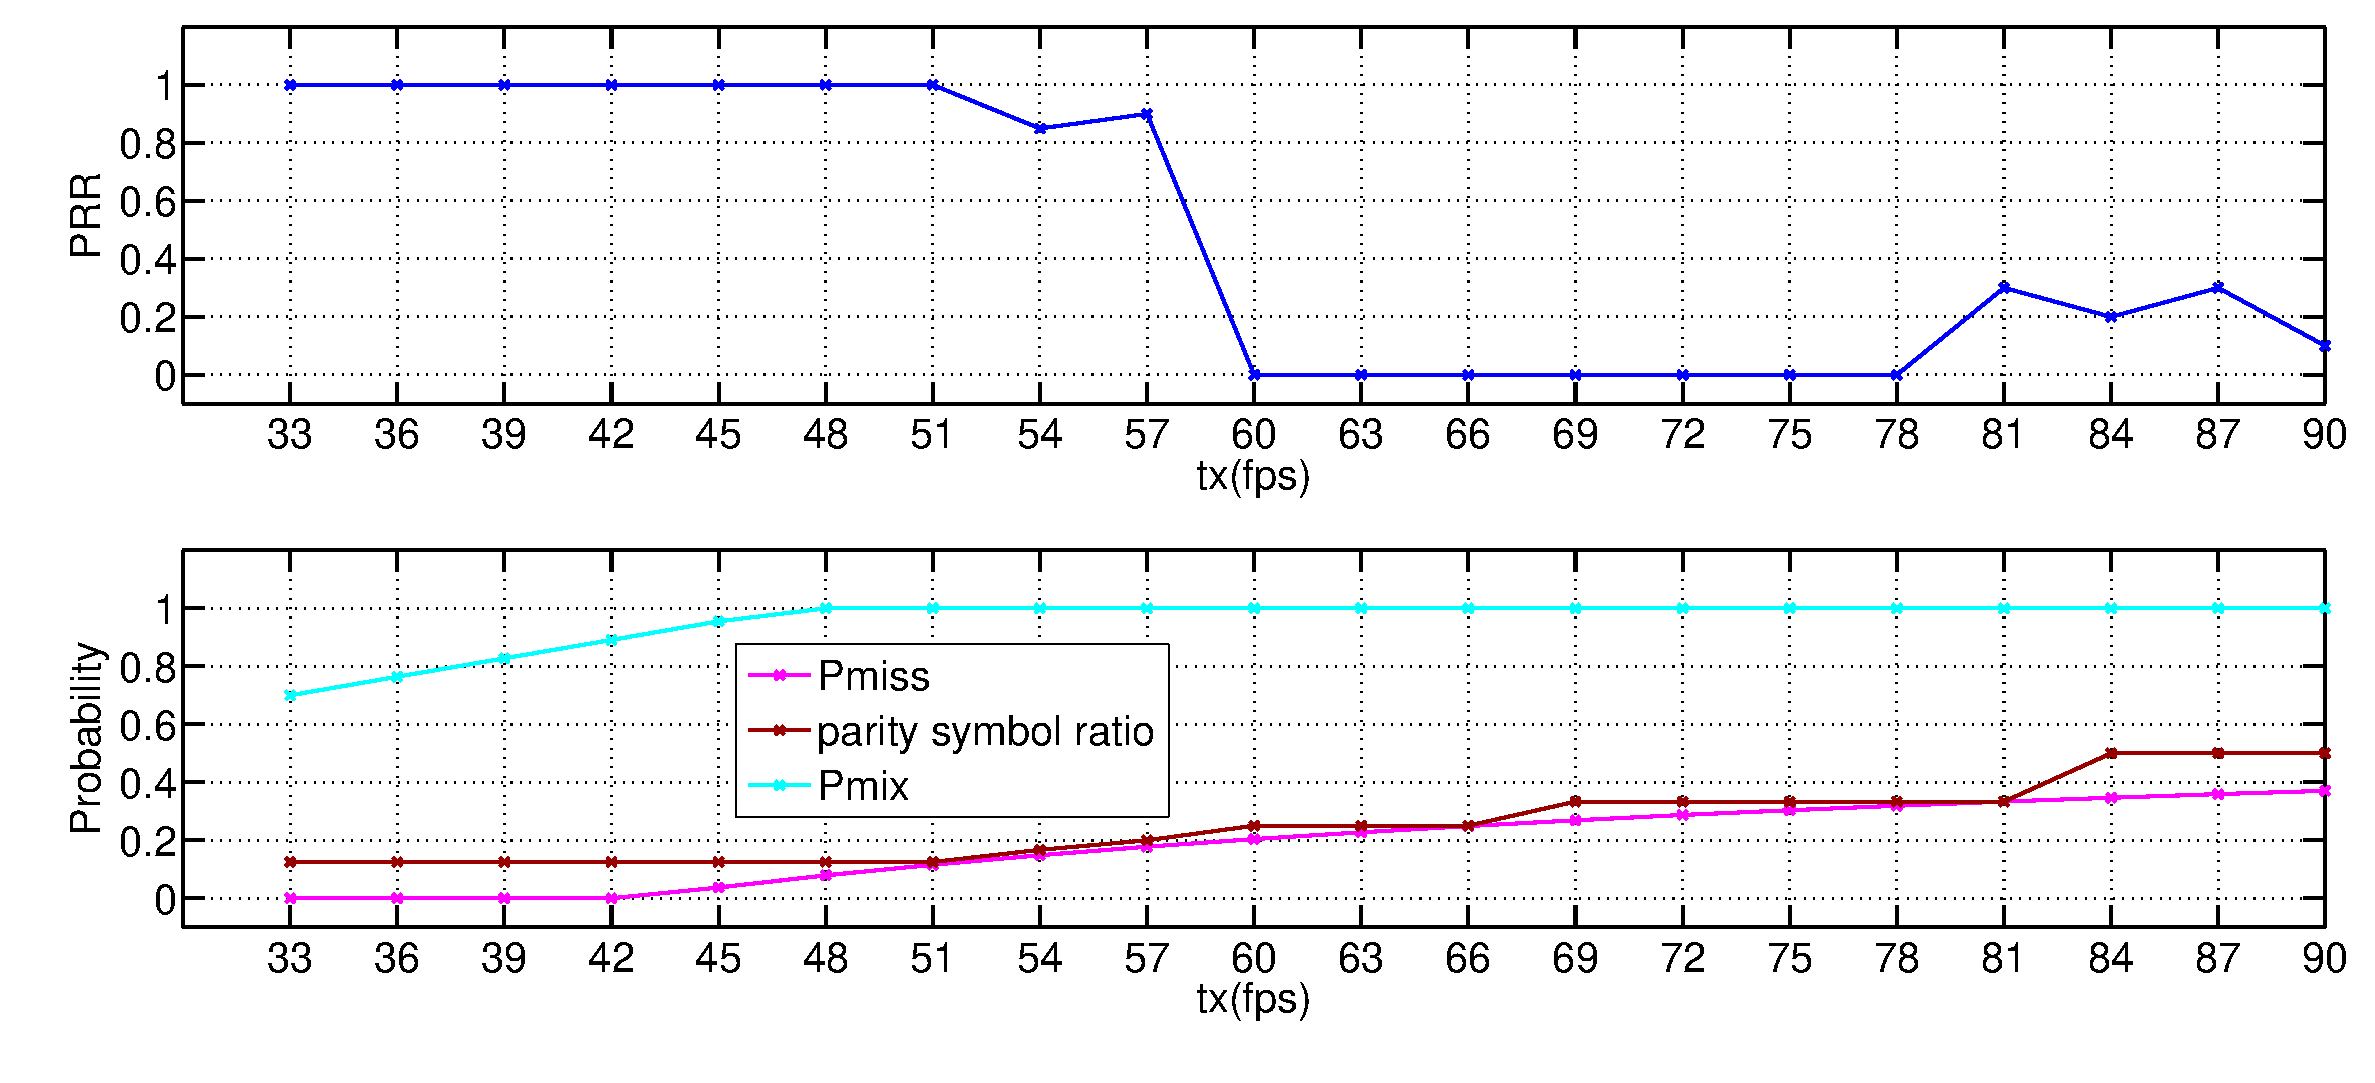
\includegraphics[scale=0.2]{fig/exp3_iphone5s_new.eps}
  \caption{Result of iPhone5s under different transmitting frame rate.}
  \label{fig:exp3_2}
\end{figure}

\autoref{fig:exp3_2} shows the result of iPhone5s. Compared to Flea3, $P_{mix}$ grows faster while $P_{miss}$ grows slower. We can see that PRR reaches 0 at 60 fps. We analyzed the data and found that $P_{miss}$ meets our expectation at this transmitting frame rate but the distribution of the missing symbols is uneven. The two missing symbols can be found in three consecutive frames, which means the parity symbol ratio is not sufficient. To address the issue, we increase the parity symbol ratio to 0.5 after 60 fps and \autoref{fig:exp3_3} shows the modified result. The PRR is above 80\% until reaches the transmitting frame rate of 81 fps. We can see that both Flea3 and iPhone5s can have high PRR when the transmitting frame rate is lower than 81 fps.

We can see the throughput line grows with a trend - at the time the parity symbol ratio increases, the throughput would stay the same or drop a little. The maximum throughput of Flea3 happens at 78 fps, and the throughput has increased by 1.2 times and reaches 18 bytes per second. The maximum throughput of iPhone5s happens at 51 fps, and the throughput has increased by 1.28 times and reaches 19.25 bytes per second.

\begin{figure}[!htb] 
 %\centering
  \hspace{-2em}
  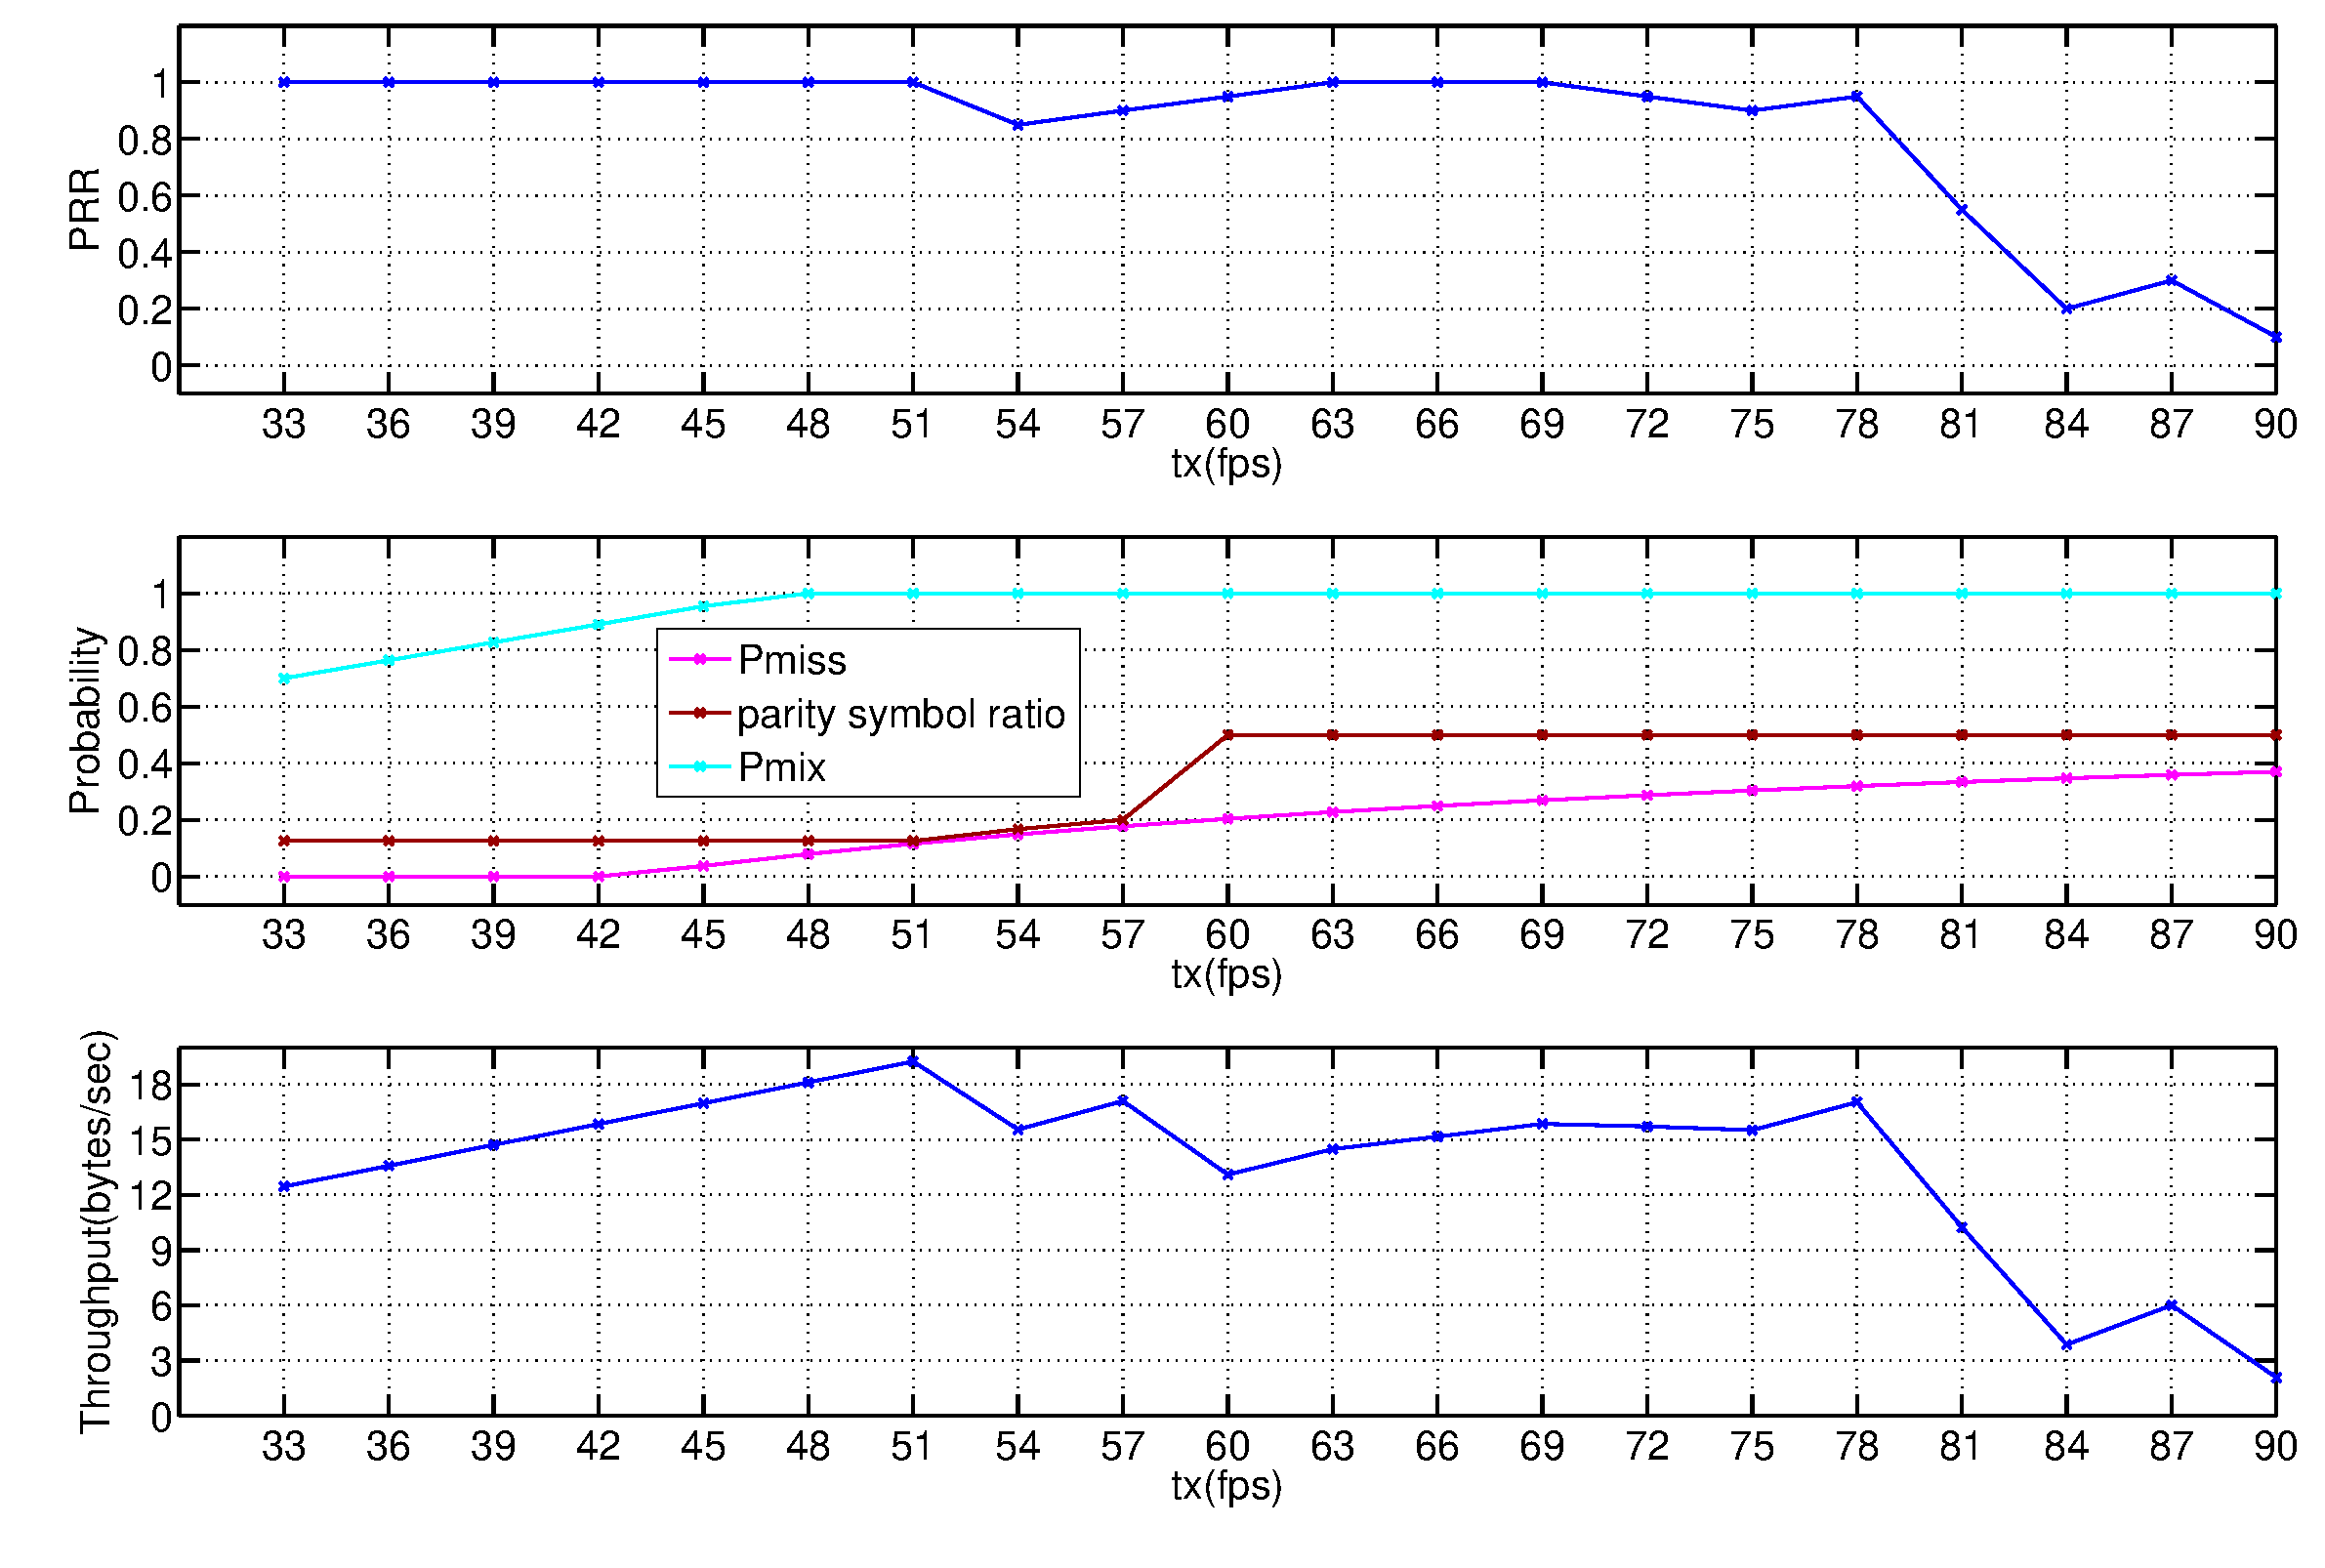
\includegraphics[scale=0.2]{fig/exp3_iphone5s_new_modify.eps}
  \caption{Modified Result of iPhone5s under different transmitting frame rate.}
  \label{fig:exp3_3}
\end{figure}

\subsection{Performance under Different LED Size in the Image}

So far, we have considered the factors of transmitting frame rate, receiving frame rate and the read-out time of the camera. There is one more factor - the image height, which may affect $P_{miss}$ and $P_{mix}$. Thus, in this experiment, we try to change the height of the LED in the received image.
There are two methods to do so, one is use the same setting with the previous experiments (which let the LED light full of the image) and simply crop the image into the height we want. The other is to move the receiver from near to far. We choose the latter method. When we get far away from the LED, although the intensity of light and the detection of the LED boundary may also cause some decoding error, we think the latter method exhibits a setting closer to the real situation. 

We use the height (pixel) of the LED in the received image as our X-axis in \autoref{fig:exp4_1}. The transmitting frame rate is configured to 30 fps. We use two cameras in this experiment. The Flea3 has a fixed receiving frame rate at 30 fps. The iPhone5s is at 29.98 fps on average. We only use the third setting in this experiment. As to how far away we can reach, it depends on the sensor size of the camera, the focal length of the lens, and the size of the LED. \autoref{tab:camera_para} lists the parameters of the cameras we use in the experiment. If we know all the above parameters, the distance from the LED to the camera is proportional to:

\begin{equation}
	distance (cm) \propto \frac{focal\_length (mm) * LED\_height (mm) * image\_height (pixels)}{LED\_height (pixels) * sensor\_height (mm)} 
	\qquad \textrm{.}
\end{equation} 

We also provide a comparison in ~\autoref{tab:comp_dis}, showing the relationship between the distance and LED height in the received image of Flea3 and iPhone5s. The real LED height we use in the experiment is 4.7 cm. In the table, we can see if the LED object in the image is around 500 pixel, the distance from the object to the Flea3 can be half a meter, while the iPhone5s can only be 15 centimeters. However, if the size of the image area illuminated by the light becomes bigger, (For transmitter-end, we can simply use the lampshade to enlarge the light range. For receiver-end, we can use the reflected light from surrounding areas, such as a wall.) we can further lift the distance limitation. 

\begin{table}[!htb]
\centering
\caption{Camera parameters of Flea3 and iPhone5s.}
  %large
  \begin{tabular}{lcc}
  \hline Parameters & Flea3 & iPhone5s \\
  \hline 
  \hline Camera Sensor Format & 1/2.5" & 1/3" \\
  \hline Image Height(pixel) & 1080 & 1080\\
  \hline Pixel Size($\mu$m) & 1.55 & 1.5 \\
  \hline Focal Length(mm) & 16 & 4.21 \\
  \end{tabular}
  \label{tab:camera_para} 
\end{table}

\autoref{fig:exp4_setup} shows a photo illustrating the experimental setup. Note that we still have a limitation that the transmitting symbol in the received image need to occupy at least two black-white strips for detecting the signal period. For example, symbol with the largest strip width received from Flea3 is 58 pixel, so the image area need to have at least a height of 232 pixel. It means if the height of LED in the received image is smaller than 232 pixel, then the received symbol cannot be decoded.

\begin{table}[!htb]
\centering
\caption{Distance table of Flea3 and iPhone5s.}
  %\large
  \hspace{-2em}
  \tabcolsep=0.11cm
  \begin{tabular}{lcccccccccc}
  \hline LED height in image (pixel) & 1000 & 900 & 800 & 700 & 600 & 500 & 400 & 300 & 200 & 100 \\
  \hline 
  \hline Flea3 distance (cm) & 48.5 & 53.9 &60.6& 69.3 &80.9& 97.0& 121.3 &161.7 &242.6 &485.2\\
  \hline iPhone5s distance (cm) & 7.75& 8.61& 9.68& 11.07& 12.91& 15.49& 19.36& 25.82& 38.73& 77.46 \\
  \end{tabular}
  \label{tab:comp_dis} 
\end{table}

\begin{figure}[!htb]
  \centering
  %\hspace{-5em}
  \includegraphics[scale=0.075]{fig/exp4_setup.JPG}
  \caption{Experimental setup photo.}
  \label{fig:exp4_setup}
\end{figure}

\begin{figure}[!htb] 
 %\centering
  %\hspace{-3em}
  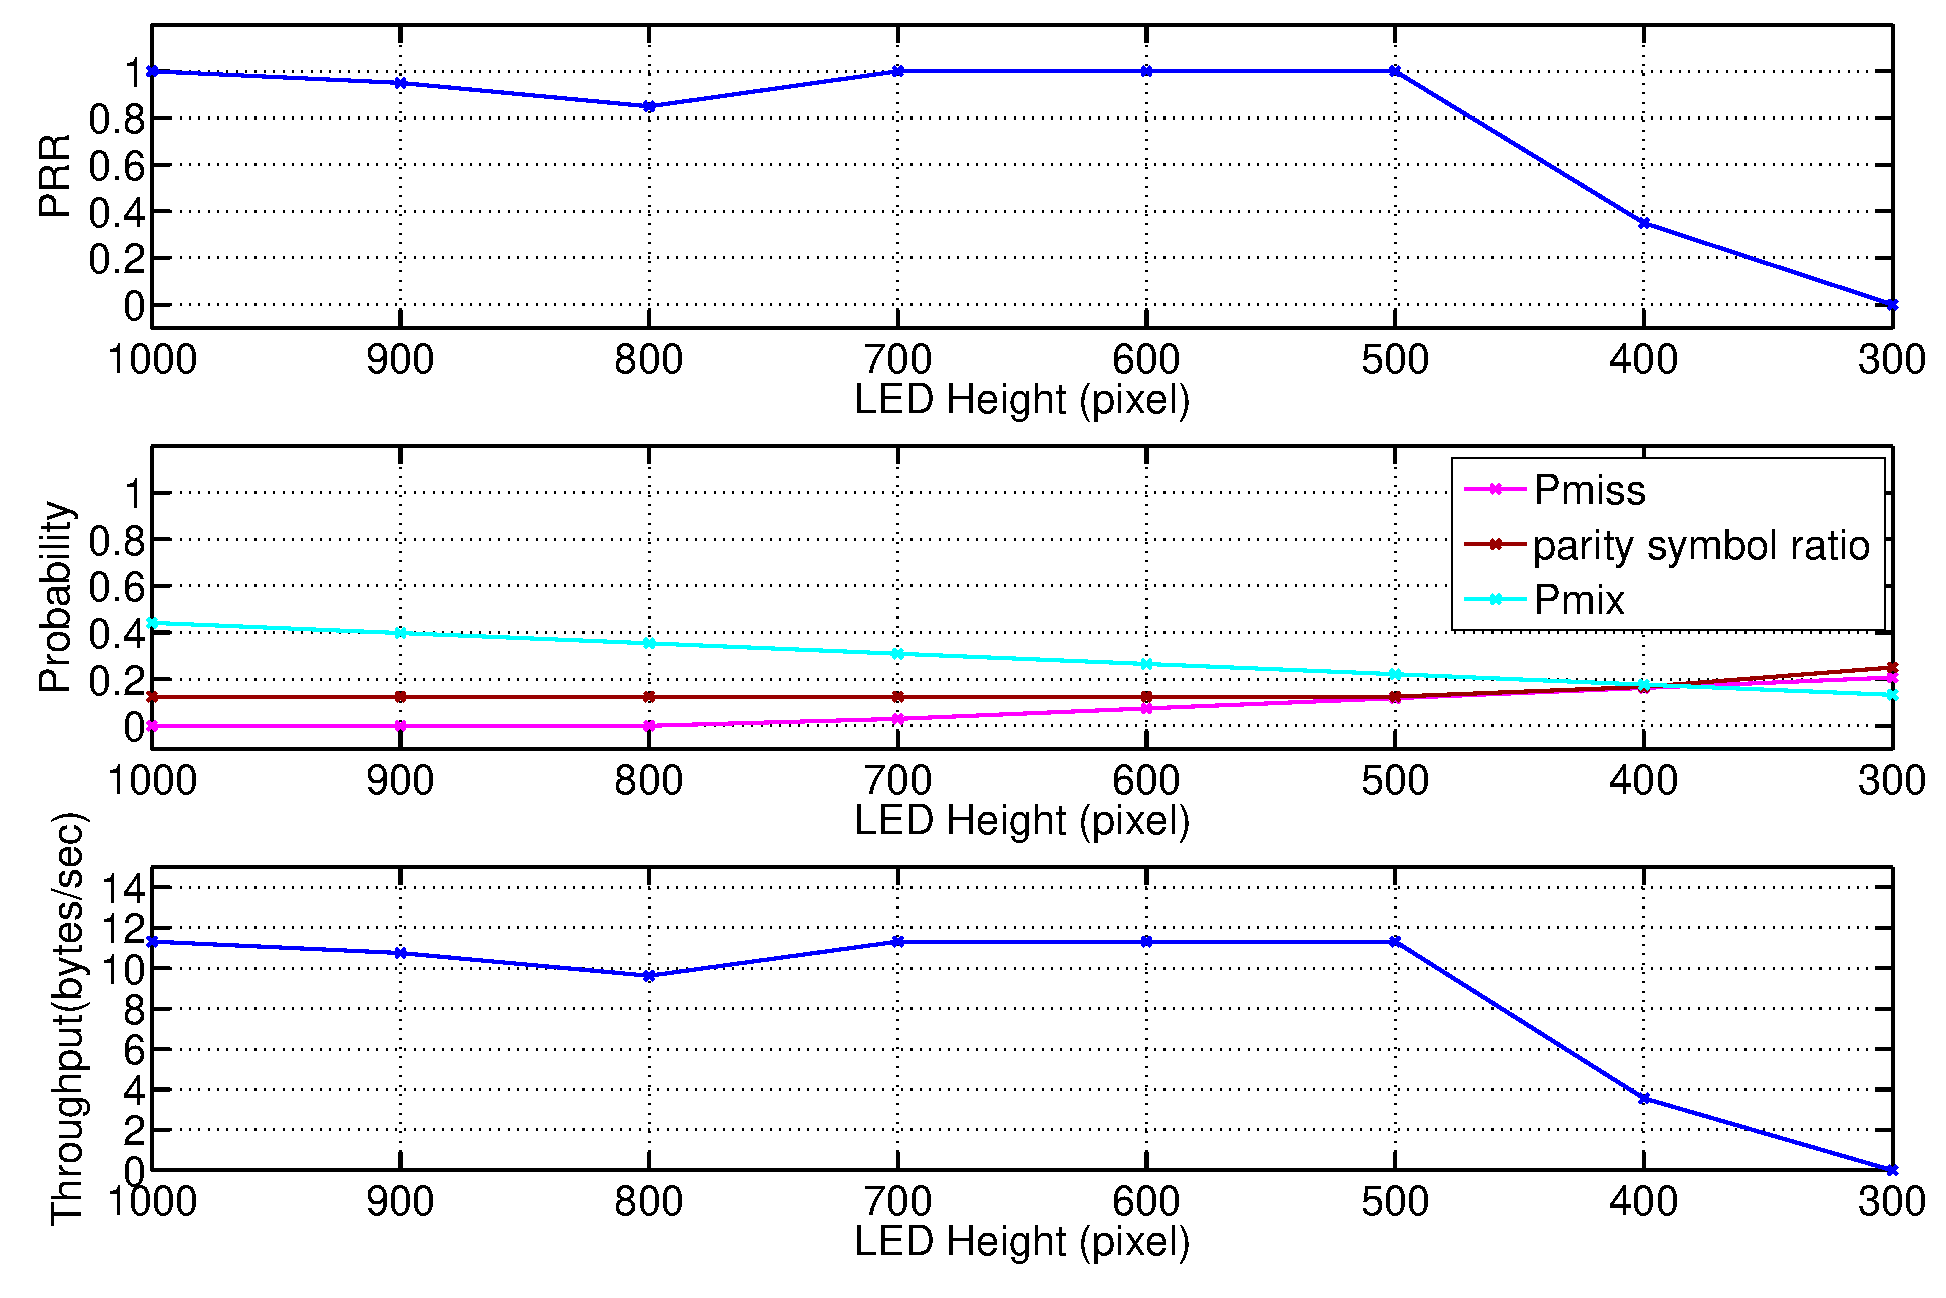
\includegraphics[scale=0.25]{fig/exp4_flea_new.eps}
  \caption{Result of Flea3 under different LED height.}
  \label{fig:exp4_1}
\end{figure}
\begin{figure}[!htb] 
 %\centering
  %\hspace{-3em}
  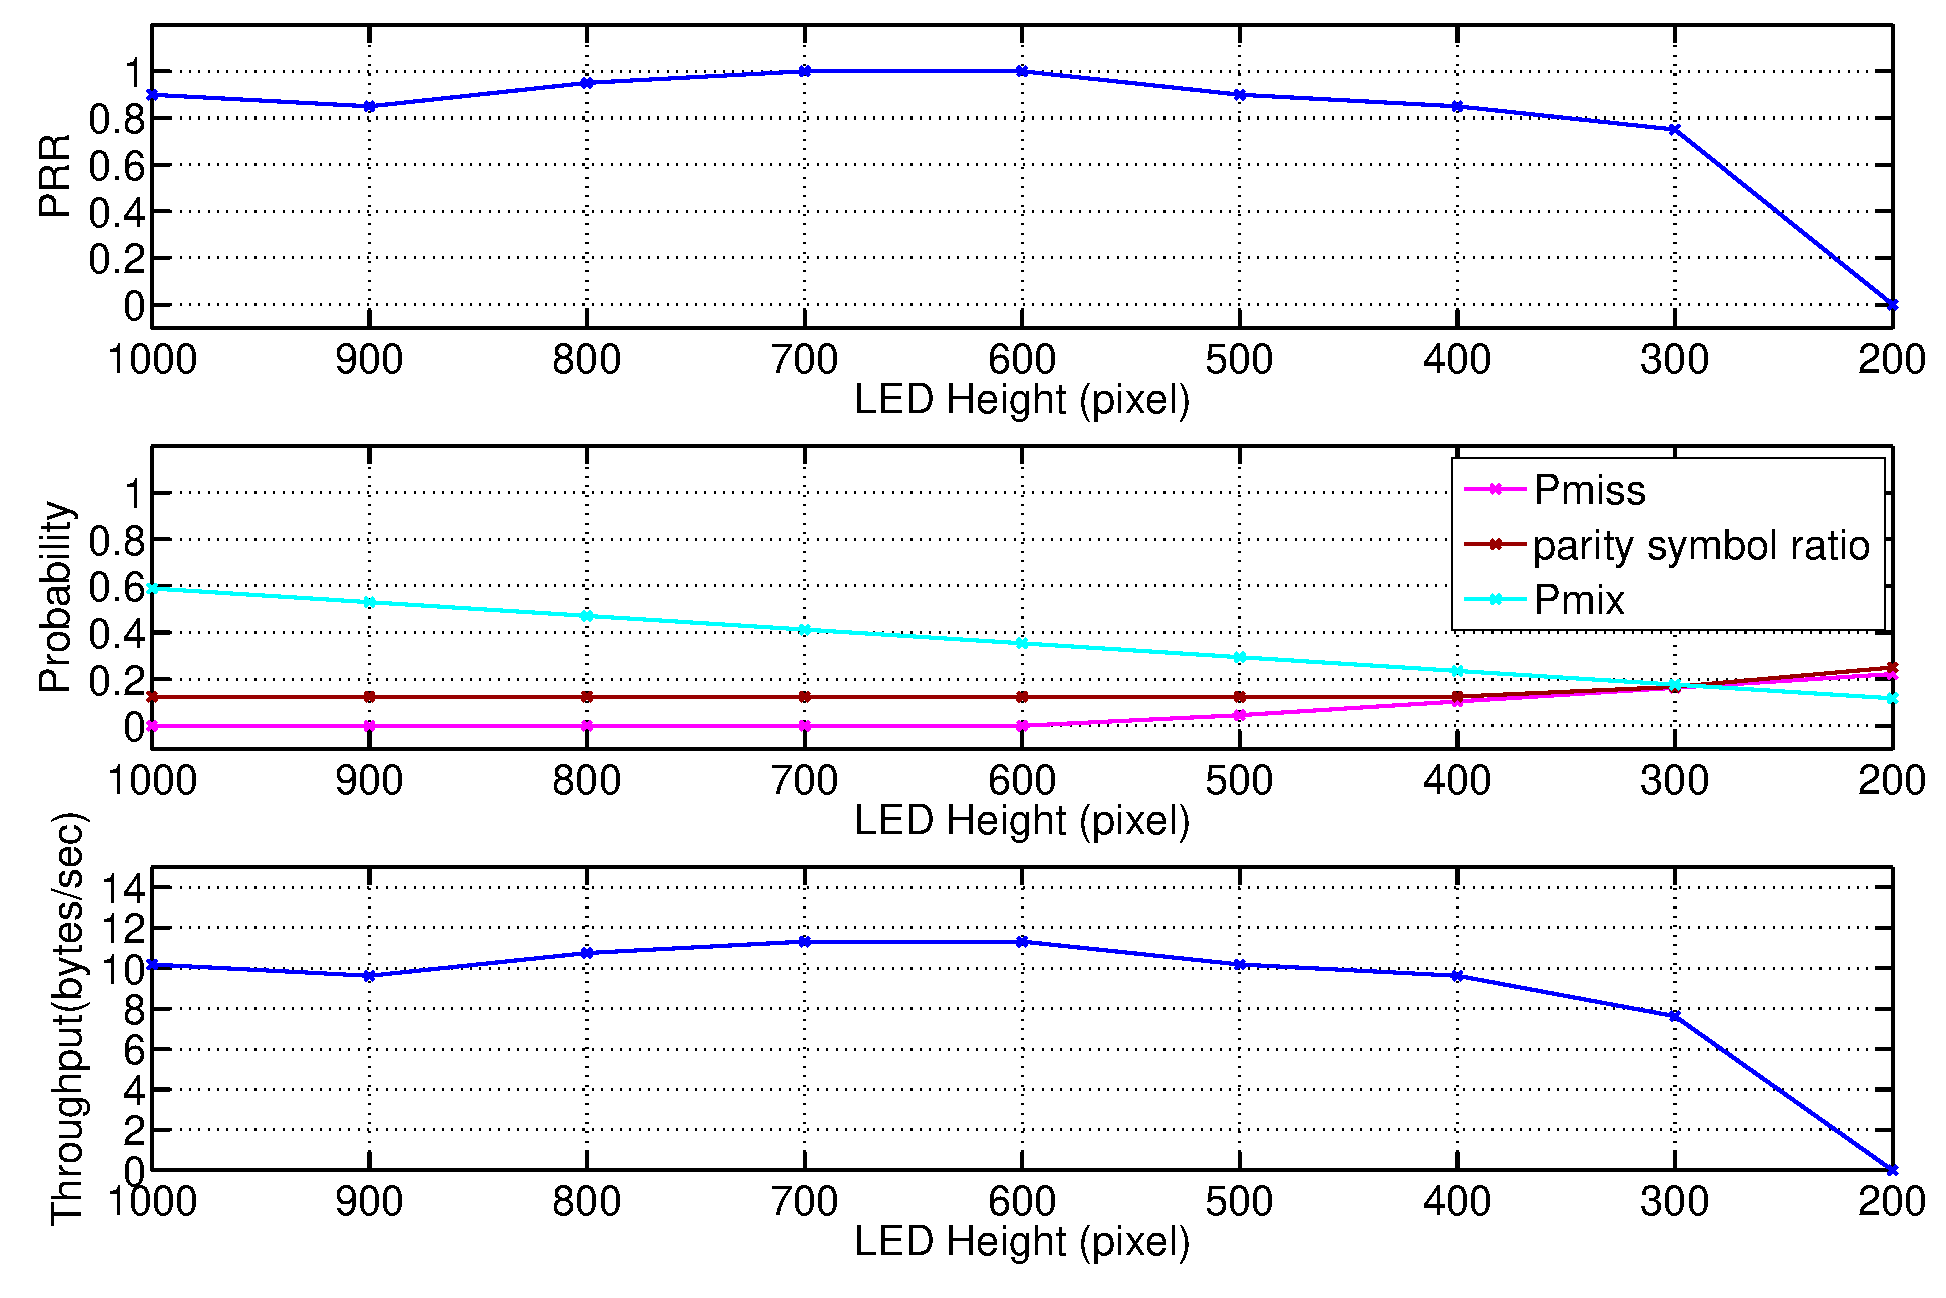
\includegraphics[scale=0.25]{fig/exp4_iphone5s_new.eps}
  \caption{Result of iPhone5s under different LED height.}
  \label{fig:exp4_2}
\end{figure}

\autoref{fig:exp4_1} shows the results of Flea3. As the LED object in the image becomes small, $P_{mix}$ slightly goes down, and $P_{miss}$ slightly goes up. Note that $P_{miss}$ here is not caused by the whole missing symbol in the received image. It means that the transmitting symbol in the received image is too short to be decoded. This happens when the symbol delimiter appears in the received image and the upper part and lower part of the symbol in the image do not have enough pixel width. We can see when the LED height is around 400 pixel, the PRR starts to drop. When the LED height is below 400 pixel, it cannot be decoded at all. Although $P_{mix}$ is not very high, the symbol delimiter can always appear in the consecutive frames together since the transmitting frame rate and the receive frame rate are close, consecutive symbol losses are observed. Therefore, it does not work even if we use a higher parity symbol ratio. 

iPhone5s, as shown in \autoref{fig:exp4_2}, due to its longer read-out time and shorter time gap between receiving frames, $P_{miss}$ is relatively smaller. Thus, when the LED has a height of around 300 pixel in the image, the transmission can still be received. The PRR is about 75\%.
 
 We can see both Flea3 and iPhone5s can achieve 9.5 $\sim$ 12 bytes per second when the LED height is above 500 pixel. As the LED object in the image becomes small, the throughput decreases significantly; due to both a smaller PRR and a large parity symbol ratio.

\subsection{Time Measurement of Real-time iOS Decoder App}
\label{sec:ios_eval}
%(needed if preview mode is not equal to video mode)
%(Figure: x:tx/rx ratio, y:PRR, color line:mode, for iphone5s app)

We have shown that our system work well for cameras on mobile devices. In this subsection, we want to know whether the decoding process can be executed in real-time with smartphone processors, we also implement an iOS decoding app, running on iPhone5s.

We use the AV Foundation framework, which provides an Objective-C interface for managing and playing audio-visual media in iOS applications. The application uses multiple threads. One thread obtains the frame buffers captured by the camera, and put the image buffers into the queue to be processed. The other thread takes the frame at the front of the queue and decodes it in real time without saving the image. Decoding results for the frame will be shown on the phone screen. \autoref{fig:ios_gui} shows the GUI of the iOS application; one can first touch the screen where the light locates to lock the focus and the exposure time. After pressing start button, the application will start to detect the LED location and decode the message.

\begin{figure}[!htb]
  \centering
  \includegraphics[scale=0.25]{fig/ios_gui3.png}
  \caption{iOS application GUI}
  \label{fig:ios_gui}
\end{figure}

%\subsection{Optimizations for real-time processing}
Since we have set the FrameDuration of the captured video data output (for example, we set the video to 30 fps), we need to make sure that we have enough time to process a frame within one FrameDuration.

To optimize the processing time, we first add the optimization level of Apple LLVM 5.1 compiler as "-Os", generating a faster and smaller executable.

Next, we time individual operations to assess their computational complexity. We found that the majority of the processing time happens when we try to get the frame buffer and convert it to the UIImage, then convert the UIImage to the OpenCV Mat type. This step takes about 0.04 sec, which is greater than a frame duration. To reduce the time, we directly get the pixel base address and put it into Mat. Surprisingly, the time reduces to 0.00003 sec.

Moreover, we found that when we convert RGB to gray scale, it also costs about 0.02 sec. To reduce the time, we change the video output pixel format to YUV color space, and use the luminance(Y) channel as the gray scale value. As a result, we save 0.02 sec.

After a series of optimizing steps, the total processing time of a frame is about 0.007 sec which is less than $1/30$ sec. Since our current implementation already meets the real-time target, we do not explore further optimizations, even though some operations could be sped up more.
 \autoref{tab:ios_time} lists the time taken for each operation.

\begin{table}[!htb]
\centering
\caption{Processing time breakdown in ms}
        %\tabcolsep=1cm
        %\large
        \begin{tabular}{lc}
        \hline Operation & time(ms) \\ \hline \hline
        Image Buffer to Mat Conversion & 0.03 \\
        Symbol Delimiter Detection & 3.25 \\
        YIN Period Detection & 3.74 \\
        GUI Text Output & 0.04 \\
        \hline
        Total & 7.06 \\
        \hline
        \end{tabular}
        \label{tab:ios_time}
\end{table}